\documentclass[12pt,a4paper]{article}
\usepackage{amssymb}
\usepackage{amsthm}
\usepackage{fontspec, xunicode, xltxtra}
\usepackage[slantfont, boldfont]{xeCJK}
\usepackage{titlesec}
\usepackage{indentfirst}
\usepackage{enumerate}
\usepackage{multicol}
\usepackage{multirow}
\usepackage[fleqn]{amsmath}
\usepackage{xcolor}
\usepackage{clrscode3e}
\usepackage{listings}
\usepackage{graphicx}
\usepackage{fancyhdr}
%\usepackage{algorithm}
%\usepackage{algorithmic}
%\usepackage{amsmath}
%\usepackage{sectsty}
%\usepackage{picinpar}
%\usepackage{bm}
%\usepackage[boxed,linesnumbered]{algorithm2e}


\setCJKmainfont[BoldFont={Adobe Heiti Std}, ItalicFont={Adobe Kaiti Std}]{Adobe Song Std}
\setCJKmonofont{Adobe Fangsong Std}
\setmainfont[Mapping=tex-text]{Liberation Serif}
\setsansfont{Liberation Sans}
\setmonofont{Bitstream Vera Sans Mono}
\punctstyle{kaiming}
\pagestyle{fancy}
\fancyhead{}
\fancyfoot{} % clear all fields
\fancyfoot[LF]{Copyright by Yinyanghu}
\fancyfoot[RF]{\thepage}
\renewcommand{\footrulewidth}{0.4pt}
\renewcommand{\headrulewidth}{0.0pt}
%\setCJKfamilyfont{kai}{KaiTi}
%\setCJKfamilyfont{hei}{SimHei}
%\setCJKmainfont{SimSun}


%\newcommand{\kai}{\CJKfamily{kai}}
%\newcommand{\hei}{\CJKfamily{hei}}
%\newcommand\TT{\rule{0pt}{2.6ex}}
%\newcommand\BB{\rule[-1.2ex]{0pt}{0pt}}



\newcommand\abs[1]{\left\lvert #1 \right\rvert}
\newcommand\floor[1]{\left\lfloor #1 \right\rfloor}
\newcommand\ceil[1]{\left\lceil #1 \right\rceil}
\setlength{\parindent}{2.5em}

\renewcommand{\labelenumi}{\bfseries{\alph{enumi}.}}
\renewcommand{\labelenumii}{\bfseries{\arabic{enumii}.}}




\begin{document}

\title{The solutions to the book \\ ``Introduction to Algorithm, 3rd Edition''}
\author{Jian Li \\ Computer Science \\ Nanjing University, China}
\date{2011}
\maketitle
\pagebreak

\section*{I Foundations}
\pagebreak

\section*{Chapter 1}

\section{Comparison of running times}

Table \ref{runtime} shows the solution.
$\lg(n)$ is $\log(n)$ base 2.
And we also assume that there are 30 days in a month and 365 days in a year.

\paragraph{Note} Thanks to \href{https://github.com/Qumeric}{Valery Cherepanov(Qumeric)} who reported an error in the previous edition of solution.

\begin{table}
\resizebox{\textwidth}{!}{
\begin{tabular}{c|c|c|c|c|c|c|c}
        & 1 second & 1 minute & 1 hour & 1 day & 1 month & 1 year & 1 century\\\hline
    $\lg(n)$ & $2^{10^6}$ & $2^{10^6 \cdot 60}$ & $2^{10^6 \cdot 60 \cdot 60}$ & $2^{10^6 \cdot 60 \cdot 60 \cdot 24}$ & $2^{10^6 \cdot 60 \cdot 60 \cdot 24 \cdot 30}$ & $2^{10^6 \cdot 60 \cdot 60 \cdot 24 \cdot 365}$ & $2^{10^6 \cdot 60 \cdot 60 \cdot 24 \cdot 365 \cdot 100}$\\\hline
    $\sqrt{N}$ & $(10^6)^2$ & $(10^6 \cdot 60)^2$ & $(10^6 \cdot 60 \cdot 60)^2$ & $(10^6 \cdot 60 \cdot 60 \cdot 24)^2$ & $(10^6 \cdot 60 \cdot 60 \cdot 24 \cdot 30)^2$ & $(10^6 \cdot 60 \cdot 60 \cdot 24 \cdot 365)^2$ & $(10^6 \cdot 60 \cdot 60 \cdot 24 \cdot 365 \cdot 100)^2$\\\hline
    $n$ & $10^6$ & $10^6 \cdot 60$ & $10^6 \cdot 60 \cdot 60$ & $10^6 \cdot 60 \cdot 60 \cdot 24$ & $10^6 \cdot 60 \cdot 60 \cdot 24 \cdot 30$ & $10^6 \cdot 60 \cdot 60 \cdot 24 \cdot 365$ & $10^6 \cdot 60 \cdot 60 \cdot 24 \cdot 365 \cdot 100$\\\hline
    $n\lg(n)$ & $62,746$ & $2.8 \cdot 10^6$ & $1.33 \cdot 10^8$ & $2.75 \cdot 10^9$ & $7.18 \cdot 10^{10}$ & $7.97 \cdot 10^{11}$ & $6.86 \cdot 10^{13}$\\\hline
    $n^2$ & $1,000$ & $7,746$ & $60,000$ & $293,939$ & $1.6 \cdot 10^6$ & $5.6 \cdot 10^6$ & $5.6 \cdot 10^7$\\\hline
    $n^3$ & $100$ & $391$ & $1,533$ & $4,421$ & $13,737$ & $31,594$ & $146,646$\\\hline
    $2^n$ & $20$ & $26$ & $32$ & $36$ & $41$ & $45$ & $51$\\\hline
    $n!$ & $(9, 10)$ & $(11, 12)$ & $(12, 13)$ & $(13, 14)$ & $(15, 16)$ & $(16, 17)$ & $(17, 18)$\\
\end{tabular}}
\caption{Solution to Problem 1.1}
\label{runtime}
\end{table}


\pagebreak

\section*{Chapter 2}

\section{Insertion sort on small arrays in merge sort}

\subsection{a}

The insertion sort can sort each sublist with length $k$ in $\Theta(k^2)$ worst-case time.
So sorting all $n/k$ sublists could be completed in $\Theta(k^2 \cdot n/k) = \Theta(nk)$ worst-case time.


\subsection{b}

\paragraph{Naive}
We could easily find a naive method.
Let us try to think $n/k$ sublists as $n/k$ sorted queues.
We scan all head elements of $n/k$ queues, and find the smallest element, then pop it from the queue.
The running time of each scan is $\Theta(n/k)$.
And we need pop all $n$ elements from $n/k$ queues.
So this naive method costs $n \cdot \Theta(n/k) = \Theta(n^2/k)$ time.  

\paragraph{Heap Sort}

\yin{If you do not know what the Heap Sort is, you could temporarily skip this method before you read \yang{Chapter 6: Heapsort}.}\\

Similarly, we could use a min-heap to maintain all head elements.
There are at most $n/k$ elements in the heap, so each \yin{INSERT} and \yin{EXTRACT-MIN} operation takes $\mathcal{O}(\log(n/k))$ worst-case time.
And every element enters and leaves the heap just once.
Therefore, the overall worst-case running time is $n \cdot \mathcal{O}(\log(n/k)) = \mathcal{O}(n\log(n/k))$.

\paragraph{Merge Sort}

We could use the same procedure in Merge Sort, except the base case is a sublist with $k$ elements instead.
We get the recurrence

\begin{equation}\notag
T(m) = \begin{cases}
\Theta(1) & \mbox{if } m \leq k \\
2T(m/2) + \Theta(m) & \mbox{otherwise}
\end{cases}
\end{equation}

Draw a \yang{recursion tree}, and get the result

\begin{equation}\notag
\begin{aligned}
T(n) &= 1/2 \cdot n/k \cdot 2k + 1/4 \cdot n/k \cdot 4k + \cdots + n\\
&= n\log(n/k)
\end{aligned}
\end{equation}

Therefore, the worst-case running time is $\Theta(n\log(n/k))$.


\subsection{c}

The largest value of $k$ is $\Theta(\log(n))$.
The running time is $\Theta(nk + n\log(n/k)) = \Theta(n\log(n) + n\log(n/\log(n))) = \Theta(n\log(n))$, which has the same running time as standard merge sort. 


\subsection{d}

Since $k$ is the length of the sublist, we should choose the largest $k$ that Insertion Sort can sort faster than Merge Sort on the list with length $k$.\\

In practice, \href{http://en.wikipedia.org/wiki/Timsort}{Timsort}, a hybrid sorting algorithm, use the exactly same idea with some complicated techniques.

\subsection*{Problem 2-2 Correctness of bubblesort}

\begin{enumerate}
	\item	我们需要证明$A'$是$A$的一个排列
	
	\item	{\bfseries Loop invariant:} \\
		对于每次开始迭代时,$A[j]=\min{\{ A[k]:j \leq k \leq n \}}$,并且,显然$A[j \twodots n]$是初始时$A[j \twodots n]$的一个排列 \\
		{\bfseries Initialization:} \\
		初始时,$j=n$,$A[j \twodots n]$ 仅有一个元素 $A[n]$,循环不变式显然成立 \\
		{\bfseries Maintenance:} \\
		根据循环不变式,$A[j]$是$A[j \twodots n]$的最小元素;如果$A[j - 1] > A[j]$,那么通过交换$A[j]$ 和$A[j - 1]$,使得$A[j - 1]$是$A[j - 1 \twodots n]$的最小值;有于在迭代开始之前,$A[j \twodots n]$是初始时$A[j \twodots n]$的一个排列,而在迭代中仅仅是交换了$A[j - 1]$和$A[j]$,所以$A[j - 1 \twodots n]$必然也是初始时$A[j - 1 \twodots n]$的一个排列;进入下一次迭代之前,$j$的值减小为$j - 1$ \\
		{\bfseries Termination:} \\
		当$j = i$时,循环结束;$A[i]=\min{\{ A[k]:i \leq k \leq n \}}$,并且$A[i \twodots n]$是初始时$A[i \twodots n]$的一个排列
		
	\item	{\bfseries Loop invariant:} \\
		对于每次开始迭代时,$A[1 \twodots i - 1]$包含初始时$A[1 \twodots n]$的最小的$i - 1$个元素,并且$A[1] \leq A[2] \leq \twodots \leq A[i - 1]$,而$A[i \twodots n]$包含初始时$A$中剩余的$n - i + 1$个元素 \\
		{\bfseries Initialization:} \\
		初始时,$i=1$,$A[1 \twodots i - 1]$ 是空集,循环不变式显然成立 \\
		{\bfseries Maintenance:} \\
		根据循环不变式,$A[1 \twodots i - 1]$包含初始时$A[1 \twodots n]$的最小的$i - 1$个元素,并且$A[1] \leq A[2] \leq \twodots \leq A[i - 1]$;而执行lines 2-4使得$A[i]$是$A[i \twodots n]$中的最小的一个,所以现在$A[1 \twodots i]$是初始时$A[1 \twodots i]$中元素的非递减排列;$A[i + 1 \twodots n]$包含初始时$A$中剩余的$n - i$个元素\\
		{\bfseries Termination:} \\
		当$i = n$时,循环结束;$A[1 \twodots i - 1]$即$A[1 \twodots n - 1]$是初始时$A[1 \twodots n - 1]$的非递减排列,且包含$A$中最小的$n - 1$个元素;显然,$A[n]$是$A$中最大的元素,所以$A[1 \twodots n]$是初始$A$排序后的序列
	\item	Bubble Sort最坏运行时间为$\Theta(n^2)$,和Insertion Sort的运行时间一样
\end{enumerate}


\subsection*{Problem 2-3 Correctness of Horner’s rule}

\begin{enumerate}
	\item	$\Theta(n)$ 
	\item	朴素算法的运行时间为$\Theta(n^2)$ \\
		\begin{codebox}
		\Procname{$\proc{Naive-Polynomial-Evaluation}(P(x), x)$}
		\li	$\id{y} \gets 0$
		\li	\For $i \gets 0$ \To $n$
		\li	\Do
				$\id{t} \gets 1$
		\li		\For $j \gets 1$ \To $i$
		\li		\Do
					$\id{t} \gets \id{t} \cdot x$
				\End
		\li		$\id{y} \gets \id{y} + \id{t} \cdot a_i$
			\End
		\li	\Return $\id{y}$
		\end{codebox}		
		
	\item	\begin{equation} \notag
		y = \sum_{k = 0}^{n}a_kx^k
		\end{equation}
		(Omit!)
	\item	(Omit!)
\end{enumerate}


\subsection*{Problem 2-4 Inversions}

\begin{enumerate}

	\item	$(1, 5), (2, 5), (3, 5), (4, 5), (3, 4)$
	\item	$\{n, n - 1, n - 2, \twodots, 2, 1\}$ \\
		总共$\binom{n}{2}=n(n-1)/2$对inversions
	\item	Insertion-Sort每交换一对元素,就消除一对原有序列中的inversion,所以所以Insertion-Sort的运行时间和inversions的对数是同数量级的
	\item	$N$个元素组成的序列,最坏运行时间为$\Theta(n\log{n})$,找出序列inversions的对数 \\
		\begin{codebox}
		\Procname{$\proc{Count-Inversions}(A, left, right)$}
		\li	$\id{inversions} \gets 0$
		\li	\If $left < right$
		\li	\Then
				$mid \gets \lfloor (left + right) / 2 \rfloor$
		\li		$\id{inversions} \gets \id{inversions} + \proc{Count-Inversions}(A, left, mid)$
		\li		$\id{inversions} \gets \id{inversions} + \proc{Count-Inversions}(A, mid + 1, right)$
		\li		$\id{inversions} \gets \id{inversions} + \proc{Merge-Inversions}(A, left, mid, right)$
			\End
		\li	\Return $\id{inversions}$
		\end{codebox}
		
		
		\begin{codebox}
		\Procname{$\proc{Merge-Inversions}(A, left, mid, right)$}
		\li	$n_1 \gets mid - left + 1$
		\li	$n_2 \gets right - mid$
		\li	Let $L[1 \twodots n_1+1]$ and $R[1 \twodots n_2 + 1]$ be new arrays
		\li	\For $i \gets 1$ \To $n_1$
		\li	\Do
				$L[i] \gets A[left + i - 1]$
			\End
		\li	\For $i \gets 1$ \To $n_2$
		\li	\Do
				$R[i] \gets A[mid + i]$
			\End
		\li	$L[n_1 + 1] \gets R[n_2 + 1] \gets \infty$
		\li	$i \gets j \gets 1$
		\li	$\id{inversions} \gets 0$
		\li	$\id{counted} \gets \const{False}$
		\li	\For $k \gets left$ \To $right$
		\li	\Do
				\If $\id{counted} \gets \const{False}$ and $L[i] > R[j]$
		\li		\Then
					$\id{inversions} \gets \id{inversions} + n_1 - i + 1$
		\li			$\id{counted} \gets \const{True}$
				\End
		\li		\If $L[i] \leq R[j]$
		\li		\Then
					$A[k] \gets L[i]$
		\li			$i \gets i + 1$
		\li		\ElseNoIf
					$A[k] \gets R[j]$
		\li			$j \gets j + 1$
		\li			$\id{counted} \gets \const{False}$
				\End
			\End
		\li	\Return $\id{inversions}$
		\end{codebox}
		
		Answer = Count-Inversions(A, 1, n) \\
		算法的最坏运行时间与Merge-Sort相同,即$\Theta(n\log{n})$
\end{enumerate}



\pagebreak


\section*{Chapter 3}

\subsection*{Problem 3-1 Asymptotic behavior of polynomials}
(Omit!)


\subsection*{Problem 3-2 Relative asymptotic growths}

\begin{lrbox}{\tablebox}
	\begin{tabular}{c  c | c | c | c | c | c |}
		$A$ & $B$ & $\mathcal{O}$ & $o$ & $\Omega$ & $\omega$ & $\Theta$ \\\hline
		$\log^k{n}$ & $n^{\epsilon}$ & Yes & Yes & No & No & No \\\hline
		$n^k$ & $c^n$ & Yes & Yes & No & No & No \\\hline
		$\sqrt{n}$ & $n^{\sin{n}}$ & No & No & No & No & No \\\hline
		$2^n$ & $2^{n/2}$ & No & No & Yes & Yes & No \\\hline
		$n^{\log{c}}$ & $c^{\log{n}}$ & Yes & No & Yes & No & Yes \\\hline
		$\log{n!}$ & $\log{n^n}$ & Yes & No & Yes & No & Yes \\\hline
	\end{tabular}
\end{lrbox}

\begin{center}
\resizebox{0.7\textwidth}{!}{\usebox{\tablebox}}
\end{center}


\subsection*{Problem 3-3 Ordering by asymptotic growth rates}
\begin{enumerate}

\item	$f(n)$增长率级别如下表: 
	\begin{lrbox}{\tablebox}
		\begin{tabular}{| l | l | l | l | l | l |} \hline
			$2^{2^{n + 1}}$ & $2^{2^n}$ & $(n + 1)!$ & $n!$ & $e^n$ & $n \cdot 2^n$ \\\hline
			$2^n$ & $(3/2)^n$ & \multicolumn{2}{l |}{$n^{\log{\log n}} = (\log n)^{\log n}$} & $(\log{n})!$ & $n^3$ \\\hline
			\multicolumn{2}{| l |}{$4^{\log n} = n^2$} & \multicolumn{2}{l |}{$n \log n$ and $\log(n!)$} & \multicolumn{2}{l |}{$2^{\log n} = n$} \\\hline
			$(\sqrt{2})^{\log n}$ & $2^{\sqrt{2 \log n}}$ & $\log^2 n$ & $\ln n$ & $\sqrt{\log n}$ & $\ln{\ln n}$ \\\hline
			$2^{\log^* n}$ & \multicolumn{2}{l |}{$\log^* n$ and $\log^*(\log n)$} & $\log(\log^*n)$ & \multicolumn{2}{l |}{$n^{1/ \log n}$ and $1$} \\\hline
		\end{tabular}
	\end{lrbox}


	\begin{center}
	\resizebox{1\textwidth}{!}{\usebox{\tablebox}}
	\end{center}


\item	\begin{equation} \notag
		f(n)=2^{2^{(n + 1)\cdot \cos n}}
	\end{equation}

\end{enumerate}


\subsection*{Problem 3-4 Asymptotic notation properties}
\begin{enumerate}
	\item	Wrong! 显然,$n = \mathcal{O}(n^2)$,但$n^2 \neq \mathcal{O}(n)$
	\item	Wrong! 令$f(n)=n^2, g(n)=n$,则$\Theta(\min(f(n),g(n)))=\Theta(n)$,显然$f(n)+g(n)=n^2+n \neq \Theta(n)$
	\item	Right! 因为$f(n)=\mathcal{O}(g(n))$且$\log(g(n)) \geq 1, f(n) \geq 1$ when $n \rightarrow \infty$,即$f(n) \leq cg(n) \Rightarrow \log(f(n)) \leq \log(cg(n))=\log c+\log(g(n))$,令$b=\log c + 1$,则$\log c+\log(g(n)) \leq b\log(g(n))$,即$\log(f(n))=\mathcal{O}(\log(g(n)))$
	\item	Wrong! 令$f(n)=2n, g(n)=n$,我们有$f(n)=\mathcal{O}(g(n))$但$2^{f(n)}=2^{2n} \neq \mathcal{O}(2^{g(n)} = 2^n)$
	\item	Wrong! 如果$f(n) < 1$
	\item	Right! 因为对于正实数$c > 0$,$f(n) \leq cg(n) \Rightarrow 1/c \cdot f(n) \leq g(n)$
	\item	Wrong! 令$f(n)=2^n$,则$f(n)=2^n \neq \Theta(f(n/2) = 2^{\sqrt n})$
	\item	Right! $f(n) + o(f(n))=\Theta(\max(f(n), o(f(n))))=\Theta(f(n))$
\end{enumerate}


\subsection*{Problem 3-5 Variations on $\mathcal{O}$ and $\Omega$}
\begin{enumerate}
	\item	\begin{equation} \notag
			f(n)=\begin{cases}
				\mathcal{O}(g(n)) \text{ \& } \overset{\infty}{\Omega}(g(n)) & \text{if } f(n)=\Theta(g(n)) \\
				\mathcal{O}(g(n)) & \text{if } 0 \leq f(n) \leq cg(n) \\
				\overset{\infty}{\Omega}(g(n)) & \text{if } 0 \leq cg(n) \leq f(n) \text{, for infinitely many integers } n \\
			\end{cases}
		\end{equation}
		如果只有有限多个$n$使得$f(n) \geq cg(n) \geq 0$,那么当$n$趋进$\infty$时,必有$0 \leq f(n) \leq cg(n)$,即$f(n)=\mathcal{O}(g(n))$ \\
		显然,用$\Omega$替换$\overset{\infty}{\Omega}$时不成立
		
	\item	Advantage: 可以刻画所有函数之间的关系 \\
		Disadvantage: 刻画得不精确
	
	\item	For any two functions $f(n)$ and $g(n)$, we have if $f(n) = \Theta(g(n))$ then $f(n) = \mathcal{O}'(g(n))$ and $f(n) = \Omega(g(n))$ \\
		But the converse is not true
	
	\item	$\overset{\sim}{\Omega}(g(n))=\{ f(n)$ : there exist positive constants $c, k$, and $n_0$ such that $0 \leq cg(n)\log^k(n) \leq f(n)$ for all $n \geq n_0 \}$ \\
		$\overset{\sim}{\Theta}(g(n))=\{ f(n)$ : there exist positive constants $c_1, c_2, k_1, k_2$, and $n_0$ such that $0 \leq c_1g(n)\log^{k_1}(n) \leq f(n) \leq c_2g(n)\log^{k_2}(n)$ for all $n \geq n_0 \}$ \\
		For any two functions $f(n)$ and $g(n)$, we have $f(n) = \overset{\sim}{\Theta}(g(n))$ if and only if $f(n)=\overset{\sim}{\mathcal{O}}(g(n))$ and $f(n)=\overset{\sim}{\Omega}(g(n))$
\end{enumerate}


\subsection*{Problem 3-6 Iterated functions}
\begin{lrbox}{\tablebox}
	\begin{tabular}{ l  l | l |}
		$f(n)$ & $c$ & $f^*_c(n)$ \\\hline
		$n - 1$ & $0$ & $n$ \\\hline
		$\log n$ & $1$ & $\log^*(n)$ \\\hline
		$n / 2$ & $1$ & $\lceil \log n \rceil$ \\\hline
		$n / 2$ & $2$ & $\lceil \log n \rceil - 1$ \\\hline
		$\sqrt{n}$ & $2$ & $\geq \log{\log n}$ \\\hline
		$\sqrt{n}$ & $1$ & $\infty$ \\\hline
		$n^{1/3}$ & $2$ & $\geq \frac{\log{\log n}}{\log 3}$ \\\hline
		$n/\log n$ & $2$ & $\mathcal{O}(\log n)$ \\\hline
		
	\end{tabular}
\end{lrbox}


\begin{center}
\resizebox{0.4\textwidth}{!}{\usebox{\tablebox}}
\end{center}



\pagebreak


\section*{Chapter 4}

\subsection*{Problem 4-1 Recurrence examples}
\begin{enumerate}
	\item	$T(n)=\Theta(n^4)$
	\item	$T(n)=\Theta(n)$
	\item	$T(n)=\Theta(n^2 \log n)$
	\item	$T(n)=\Theta(n^2)$
	\item	$T(n)=\Theta(n^{\log_2{7}})$
	\item	$T(n)=\Theta(\sqrt{n} \log n)$
	\item	$T(n)=\Theta(n^3)$
\end{enumerate}


\subsection*{Problem 4-2 Parameter-passing costs}
\begin{enumerate}
	\item	\begin{enumerate}
			\item	$T(n)=T(n/2)+\Theta(1) \Rightarrow T(n)=\Theta(\log n)$
			\item	$T(n)=T(n/2)+\Theta(N) \Rightarrow T(n)=\Theta(N \log n)$
			\item	$T(n)=T(n/2)+\Theta(n) \Rightarrow T(n)=\Theta(n)$
		\end{enumerate}
	\item	\begin{enumerate}
			\item	$T(n)=2T(n/2)+\Theta(n) \Rightarrow T(n)=\Theta(n \log n)$
			\item	$T(n)=2T(n/2)+\Theta(N) \Rightarrow T(n)=\Theta(nN)$
			\item	$T(n)=2T(n/2)+\Theta(n) \Rightarrow T(n)=\Theta(n \log n)$
		\end{enumerate}

\end{enumerate}


\subsection*{Problem 4-3 More recurrence examples}
\begin{enumerate}
	\item	$T(n)=\Theta(n^{\log_3{4}})$
	\item	$T(n)=\Theta(n\log \log n)$
	\item	$T(n)=\Theta(n^2 \sqrt{n})$
	\item	$T(n)=\Theta(n \log n)$
	\item	$T(n)=\Theta(n \log \log n)$
	\item	$T(n)=\Theta(n)$
	\item	$T(n)=\Theta(\log n)$
	\item	$T(n)=\Theta(n \log n)$
	\item	$T(n)=\Theta(n/ \log n)$
	\item	$T(n)=\Theta(n \log \log n)$
\end{enumerate}


\subsection*{Problem 4-4 Fibonacci numbers}
\begin{enumerate}
	\item	(Omit!)
	\item	(Omit!)
	\item	无穷等比数列展开可得到
		\begin{equation} \notag
			F(z)=\sum^{\infty}_{i=0}{\frac{1}{\sqrt{5}}(\phi ^i - \hat{\phi} ^i)z^i}
		\end{equation}
	\item	因为$|\hat{\phi}| < 1$,所以当$i \rightarrow \infty$时,有$\hat{\phi}^i \rightarrow 0$,所以$F_i=\phi ^i / \sqrt{5}$ for $i>0$最接近于Fibonacci数
\end{enumerate}


\subsection*{Problem 4-5 Chip testing}
Note:当我们找到一个好的芯片的时候,所有的芯片的好坏就可以全部知道
\begin{enumerate}
	\item	我们假设有一个芯片是好的,那么因为坏的芯片数量超过一半,所以教授在测试这个芯片是否是好的时候,根据题意,所有的坏芯片可以联合起来共同欺骗教授,即说这是坏的,那么教授就会认为这是哥坏的芯片;所以当坏的芯片超过半数时,教授无法判断哪个芯片是好的
	\item	可以对$n$个芯片进行成对测试,总共$\lfloor n/2 \rfloor$对;我们将测试结果分成两组,一组是测试结果为AB同好坏的,我们称为P组;另一组是测试结果至少有一个是坏的,我们称为Q组;由于总体上good $>$ bad,且Q组必然good $\leq$ bad,所以P组必是 good $>$ bad,所以,为了找到一个好的芯片,我们可以舍弃Q组的所有芯片,而P组的芯片我们可以从每一对中任选出一个,作为下一次测试的对象,这样问题规模至少减少为原来的 $\frac{1}{2}$
	\item	$T(n)=T(n/2)+n/2 \Rightarrow T(n)=\Theta(n)$
\end{enumerate}


\subsection*{Problem 4-6 Monge arrays}
\begin{enumerate}
	\item	由定义可证
	\item	$A[2,3]=5$
	\item	若存在$f(i) > f(i + 1)$,即存在$A[i, j] + A[i + 1, k] > A[i, f(i)] + A[i + 1, f(i + 1)]$,所以不满足Monge array的定义,所以不存在$f(i) > f(i + 1)$,即$f(1) \leq f(2) \leq \twodots \leq f(m)$
	\item	由(c)易得该时间为$\mathcal{O}(m + n)$算法
	\item	$T(m)=T(m/2)+\mathcal{O}(m + n) \Rightarrow T(m)=\mathcal{O}(m + n \log m)$
\end{enumerate}



\pagebreak


\section*{Chapter 5}

\subsection*{Problem 5-1 Probabilistic counting}
\begin{enumerate}
	\item	$X_i(1 \leq i \leq n)$表示在第$i$次增加操作时计数器增加的值,$V_i$表示在$i$次增加操作后计数器表示的值 \\ \\
		$V_n=\sum_{i=1}^{n}{X_i}$ \\ \\
		$E[V_n]=E[\sum_{i=1}^{n}{X_i}]=\sum_{i=1}^{n}{E[X_i]}$ \\ \\
		而$E[X_i]=0 \cdot (1 - \frac{1}{n_{i + 1} - n_i} + (n_{i + 1}-n_i) \cdot \frac{1}{n_{i + 1} - n_i}) = 1$,即$E[V_n]=n$
	\item	$X_i$两两独立,所以$Var[V_n]=Var[X_1] + Var[X_2] + \twodots + Var[X_n]$ \\ \\
		$Var[X_i] = E[X_i^2] - E^2{[X_i]}=((0^2 \cdot \frac{99}{100}) + (100^2 \cdot \frac{1}{100})) - 1^2 = 99$ \\ \\
		所以$Var[V_n]=99n$
\end{enumerate}


\subsection*{Problem 5-2 Searching an unsorted array}
\begin{enumerate}
	\item	算法如下:
		\begin{codebox}
		\Procname{$\proc{RANDOM-SEARCH}(\id{A}, x)$}
		\li	$\id{B} \gets \emptyset$
		\li	\While $\id{B} \neq \id{A}$
		\li	\Do
				$i \gets \proc{RANDOM}(1, n)$
		\li		\If $\id{A}[i] \gets x$
		\li		\Then
					\Return $i$
				\End
		\li		$\id{B} \gets \id{B} \cup \id{A}[i]$
			\End
		\li	\Return Null
		\end{codebox}
	\item	期望在第$n$次找到$x$
	\item	期望在第$n/k$次找到$x$
	\item	期望在$\Theta(n \log n)$次找到$A$中的所有元素
	\item	Average-Case: $\frac{n+1}{2}$, Worst-Case: $n$
	\item	Average-Case:
		\begin{equation} \notag
			\sum_{i = 1}^{n - k + 1} \frac{i \binom{n - i}{k - 1}}{\binom{n}{k}} = \frac{\binom{n + 1}{k + 1}}{\binom{n}{k}} = \frac{n + 1}{k + 1}
		\end{equation}
		Worst-Case: $n - k + 1$
	\item	Average-Case:$n$, Worst-Case:$n$
	\item	$K = 0$: Worst-Case: $n$, Expected: $n$ \\ \\
		$K = 1$: Worst-Case: $n$, Expected: $\frac{n+1}{2}$ \\ \\
		For $K \geq 1$, Worst-Case: $n - k + 1$, Expected: $\frac{n + 1}{k + 1}$
	\item	Scramble-Search
\end{enumerate}



\pagebreak


\section*{II Sorting and Order Statistics}
\pagebreak

\section*{Chapter 6}

\subsection*{Problem 6-1 Building a heap using insertion}
\begin{enumerate}
	\item	No, counterexample: ${1, 2, 3}$
	\item	很明显Worst-Case的上界为$\mathcal{O}(n \log n)$,所以我们主要来证明下界 \\ \\
		\begin{equation} \notag
		\begin{aligned}
		T(n) & = \sum_{i = 1}^{n} \Theta(\lfloor \log i \rfloor) \\ & \geq \sum_{i = \lceil \frac{n}{2} \rceil}^{n} \Theta(\lfloor \log i \rfloor) \\ & \geq \sum_{i = \lceil \frac{n}{2} \rceil}^{n} \Theta(\lfloor \log(\lceil \frac{n}{2} \rceil) \rfloor) \\ & = \sum_{i = \lceil \frac{n}{2} \rceil}^{n} \Theta(\lfloor \log n - 1 \rfloor) = \Omega(n \log n)
		\end{aligned}
		\end{equation}
		所以,Worst-Case的界为$\Theta(n \log n)$		
\end{enumerate}


\subsection*{Problem 6-2 Analysis of d-ary heaps}
\begin{enumerate}
	\item	index $i$, $j$-th child $(1 \leq j \leq d)$
		\begin{codebox}
		\Procname{$\proc{D-ary-Parent}(i)$}
		\li	\Return $\lfloor (i - 2) / d + 1 \rfloor$
		\end{codebox}
		
		\begin{codebox}
		\Procname{$\proc{D-ary-Child}(i, j)$}
		\li	\Return $d(i - 1) + j + 1$
		\end{codebox}
	\item	$\Theta(\log_d n)$
	\item	和Heap-Extract-Max类似,只是在Max-Heapify中,由每次的比较2个元素找最大值,变成比较$d$个元素找最大值,所以运行时间为$\mathcal{O}(d \log_d n)$
	\item	和Max-Heap-Insert类似,运行时间为$\mathcal{O}(\log_d n)$
	\item	和Heap-Increase-Key类似,运行时间为$\mathcal{O}(\log_d n)$
\end{enumerate}


\subsection*{Problem 6-3 Young tableaus}
\begin{enumerate}
	\item
		\begin{tabular}{llll}
			2 & 3 & 4 & 5 \\
			8 & 9 & $\infty$ & $\infty$ \\
			12 & 14 & $\infty$ & $\infty$ \\
			16 & $\infty$ & $\infty$ & $\infty$ \\
		\end{tabular}
	\item	(Omit!)
	\item	类似用Max-Heapify的方法,用$\mathcal{O}(m + n)$来维护Young Tableau的结构
	\item	用$\mathcal{O}(m + n)$的时间来找到一个不存在的元素,即$\infty$;将元素插入到这个位置,然后用$\mathcal{O}(m + n)$的时间来维护Young Tableau的结构
	\item	Young-Tableau-Insert:$\mathcal{O}(n^3)$ \\
		Young-Tableau-Extract-Min:$\mathcal{O}(n^3)$ \\
		Total:$\mathcal{O}(n^3)$
	\item	注意$m \times n$Young Tableau的左下角的元素,以此元素为根,会形成一个类似Binary Search Tree的结构,算法和BST相同,所以运行时间即结构的高度$\mathcal{O}(m + n)$
\end{enumerate}



\pagebreak

\section*{Chapter 7}

\subsection*{Problem 7-1 Hoare partition correctness}
\begin{enumerate}
	\item	(Omit!)
	\item	因为当Hoare-Partition执行时,$p \leq i < j \leq r$恒成立,所以$i,j$不会访问$A[p \twodots r]$以外的元素
	\item	显然,当$i \geq j$时,Hoare-Partition结束,所以$p \leq j < r$
	\item	当Hoare-Partition结束时,有$A[p \twodots j] \leq x \leq A[j + 1 \twodots r]$
	\item	the QUICKSORT procedure to use HOARE-PARTITION 
		\begin{codebox}
		\Procname{$\proc{Quicksort'}(A, p, r)$}
		\li	\If $p < r$
		\li	\Then
				$\id{q} \gets \proc{Hoare-Partition}(A, p, r)$
		\li		$\proc{Quicksort'}(A, p, q)$
		\li		$\proc{Quicksort'}(A, q + 1, r)$
			\End		
		\end{codebox}
		
\end{enumerate}


\subsection*{Problem 7-2 Quicksort with equal element values}
\begin{enumerate}
	\item	$\mathcal{O}(n \log n)$
	\item	two methods: \\ \\
		Method 1:
		\begin{codebox}
		\Procname{$\proc{Partition'}(A, p, r)$}
		\li	$\id{x} \gets A[p]$
		\li	$\id{i} \gets p - 1$
		\li	$\id{j} \gets r + 1$
		\li	\While \const{True}
		\li	\Do
				\Repeat
		\li			$\id{j} \gets \id{j} - 1$
		\li		\Until $A[j] < \id{x}$
		\li		\Repeat
		\li			$\id{i} \gets \id{i} + 1$
		\li		\Until $A[i] > \id{x}$
		\li		\If $i < j$
		\li		\Then
					exchange $A[i]$ with $A[j]$
		\li		\ElseNoIf
					\Return $j, i$
				\End
			\End
		\end{codebox}
		
		Method 2:
		\begin{codebox}
		\Procname{$\proc{Partition'}(A, p, r)$}
		\li	$\id{i} \gets \id{j} \gets \proc{Partition}(A, p, r)$
		\li	\While $i > 1$ and $A[i - 1] \gets A[i]$
		\li	\Do
				$\id{i} \gets \id{i} - 1$
			\End
		\li	\While $j < r$ and $A[j + 1] \gets A[j]$
		\li	\Do
				$\id{j} \gets \id{j} + 1$
			\End
		\li	\Return $i, j$
		\end{codebox}
		take $\Theta(r - p)$ time
	\item	(Omit!)
	\item	因为 $\proc{Quicksort'}$的比较次数一定少于$\proc{Quicksort}$,运行时间仍然为$\mathcal{O}(n \log n)$
\end{enumerate}


\subsection*{Problem 7-3 Alternative quicksort analysis}
\begin{enumerate}
	\item	$E[X_i] = 1 / n$
	\item
		\begin{equation} \notag
			E[T(n)] = E[\sum_{q = 1}^n X_q(T(q - 1) + T(n - q) + \Theta(n))]
		\end{equation}
	\item
		\begin{equation} \notag
			E[T(n)] = \frac{2}{n} \sum_{q = 2}^{n - 1}E[T(q)] + \Theta(n)
		\end{equation}
	\item
		\begin{equation} \notag
		\begin{aligned}
			\sum_{k = 2}^{n - 1} k \log k & \leq \sum_{k = 1}^{\lceil \frac{n}{2} \rceil - 1} k \log k + \sum_{k = \lceil \frac{n}{2} \rceil}^n k \log k \\
			& \leq \frac{(\frac{n}{2})^2}{2} \log \frac{n}{2} + \frac{(\frac{n}{2} + n) \frac{n}{2}}{2} \log n \\
			& = \frac{n^2}{8} \log n - \frac{n^2}{8} + \frac{3}{8} n^2 \log n \\
			& = \frac{1}{2} n^2 \log n - \frac{n^2}{8}
		\end{aligned}
		\end{equation}
	\item	$E[T(n)] = \Theta(n \log n)$
\end{enumerate}


\subsection*{Problem 7-4 Stack depth for quicksort}
\begin{enumerate}
	\item	(Omit!)
	\item	在Worst-Case的情况下,每次$q = r$,所以对于$n$个元素的序列,Stack的深度最多为$\Theta(n)$
	\item	The worst-case stack depth is $\Theta(\log n)$, and the expected running time is $\mathcal{O}(n \log n)$
		\begin{codebox}
		\Procname{$\proc{Tail-Recursive-Quicksort'}(A, p, r)$}
		\li	\While $p < r$
		\li	\Do
				\Comment Partition and sort the small subarray first
		\li		$\id{q} \gets \proc{Partition}(A, p, r)$
		\li		\If $\id{q} - p < r - \id{q}$
		\li		\Then
					$\proc{Tail-Recursive-Quicksort'}(A, p, q - 1)$
		\li			$p \gets \id{q} + 1$
		\li		\ElseNoIf
					$\proc{Tail-Recursive-Quicksort'}(A, q + 1, r)$
		\li			$r \gets \id{q} - 1$
				\End
			\End
		\end{codebox}
\end{enumerate}


\subsection*{Problem 7-5 Median-of-3 partition}
\begin{enumerate}
	\item	$P_i = \frac{6(i - 1)(n - i)}{n(n - 1)(n - 2)}$
	\item	概率从原来的$\frac{1}{n}$增长为
		\begin{equation} \notag
			\lim_{n \rightarrow \infty} P_{\lfloor (n + 1) / 2 \rfloor} = \frac{3}{2} \cdot \frac{1}{n}
		\end{equation}
	\item
		\begin{equation} \notag
			\sum_{i = \frac{n}{3}}^{\frac{2n}{3}} P_i \approx \int_{\frac{n}{3}}^{\frac{2n}{3}} P_i = \frac{13}{27}
		\end{equation}
	\item	每次$\proc{Partition}$只增加$\mathcal{O}(1)$的操作,所以总的复杂度依然是$\Theta(n \log n)$,Median-of-3 method只影响常数时间
\end{enumerate}


\subsection*{Problem 7-6 Fuzzy sorting of intervals}
\begin{enumerate}
	\item	A randomized algorithm for fuzzy-sorting $n$ intervals
		\begin{codebox}
		\Procname{$\proc{Find-Intersection}(A, B, p, s, a, b)$}
		\li	$i \gets \proc{Random}(p, s)$
		\li	exchange $A[i]$ with $A[s]$
		\li	exchange $B[i]$ with $B[s]$
		\li	$a \gets A[s]$
		\li	$b \gets B[s]$
		\li	\For $i \gets p$ \To $s - 1$
		\li	\Do
				\If $A[i] \leq b$ and $B[i] \geq a$
		\li		\Then
					\If $A[i] > a$
		\li			\Then
						$a \gets A[i]$
		\li			\ElseIf $B[i] < b$
		\li			\Then
						$b \gets B[i]$
					\End
				\End
			\End
		\end{codebox}
		
		\begin{codebox}
		\Procname{$\proc{Partition-Right}(A, B, a, p, s)$}
		\li	$i \gets p - 1$
		\li	\For $j \gets p$ \To $s - 1$
		\li	\Do
				\If $A[j] \leq a$
		\li		\Then
					$i \gets i + 1$
		\li			exchange $A[i]$ with $A[j]$
		\li			exchange $B[i]$ with $B[j]$
				\End
			\End
		\li	exchange $A[i + 1]$ with $A[s]$
		\li	exchange $B[i + 1]$ with $B[s]$
		\li	\Return i + 1
		\end{codebox}		
		
		\begin{codebox}
		\Procname{$\proc{Partition-Left-Middle}(A, B, b, p, r)$}
		\li	$i \gets p - 1$
		\li	\For $j \gets p$ \To $r - 1$
		\li	\Do
				\If $B[j] < b$
		\li		\Then
					$i \gets i + 1$
		\li			exchange $A[i]$ with $A[j]$
		\li			exchange $B[i]$ with $B[j]$
				\End
			\End
		\li	exchange $A[i + 1]$ with $A[r]$
		\li	exchange $B[i + 1]$ with $B[r]$
		\li	\Return i + 1
		\end{codebox}			
		
		\begin{codebox}
		\Procname{$\proc{Fuzzy-Sort}(A, B, p, s)$}
		\li	\If $p < s$
		\li	\Then
				$a \gets b \gets 0$
		\li		$\proc{Find-Intersection}(A, B, p, s, a, b)$
		\li		$r \gets \proc{Partition-Right}(A, B, a, p, s)$
		\li		$q \gets \proc{Partition-Left-Middle}(A, B, b, p, r)$
		\li		$\proc{Fuzzy-Sort}(A, B, p, q - 1)$
		\li		$\proc{Fuzzy-Sort}(A, B, r + 1, s)$
			\End
		\end{codebox}
	\item	The algorithm runs in expected time $\Theta(n \log n)$ in general, but runs in expected time $\Theta(n)$ when all of the intervals overlap. Since when all of the intervals overlap, the procedure $\proc{Fuzzy-Sort}$ just calls the procedure $\proc{Find-Intersection}$ only once and then return. Therefore, the algorithm runs in expected time $\Theta(n)$.
\end{enumerate}



\pagebreak


\section*{Chapter 8}

\subsection*{Problem 8-1 Probabilistic lower bounds on comparison sorting}
\begin{enumerate}
	\item	reachable leaves: each of the $n!$ possible permutations is the input with the probability $1 / n!$ \\
		unreachable leaves: the probability is $0$
	\item	Let $d_T(x) =$ depth of node $x$ in tree $T$
		\begin{equation} \notag
		\begin{aligned}
			D(T) & = \sum_{x \in leaves(T)} d_T(x) \\ 
			& = \sum_{x \in leaves(LT)} d_T(x) + \sum_{x \in leaves(RT)} d_T(x) \\
			& = \sum_{x \in leaves(LT)} (d_{LT}(x) + 1) + \sum_{x \in leaves(RT)} (d_{RT}(x) + 1) \\
			& = \sum_{x \in leaves(LT)} d_{LT}(x) + \sum_{x \in leaves(RT)} d_{RT}(x) + \sum_{x \in leaves(T)} 1 \\
			& = D(LT) + D(RT) + k
		\end{aligned}
		\end{equation}
	\item	A decision tree $T$ with $k$ leaves that the left tree has $i$ leaves and the right tree has $k - i$ leaves.
		\begin{equation} \notag
			d(k) = \min_{1 \leq i \leq k - 1} \{ d(i) + d(k - i) + k \}
		\end{equation}
	\item	Using derivative, it's easy to have the function $i \log i + (k - i) \log (k - i)$ is minimized at $i = k / 2$ \\
		When $i = k / 2$, using Master Theorem, we have $d(k) = \Omega(k \log k)$
	\item	Let $k = n!$, then $D(T_A) \geq d(k) = \Omega(k \log k)$, therefore $D(T_A) = \Omega(n! \log n!)$
		Since the $n!$ permutations have equal probability $1 / n!$, the expected time to sort $n$ random elements is
		\begin{equation} \notag
			\frac{\Omega(n! \log (n!))}{n!} = \Omega(\log n!) = \Omega(n \log n)
		\end{equation}
\end{enumerate}


\subsection*{Problem 8-2 Sorting in place in linear time}
\begin{enumerate}
	\item	Counting-Sort
	\item	Quicksort-Partition
	\item	Insertion-Sort
	\item	(a) Yes (b) No (c) No
	\item	use $\mathcal{O}(k)$ outside the input array
		\begin{codebox}
		\Procname{$\proc{Counting-Sort}(A, k)$}
		\li	\Comment let $C[0 \twodots k]$ be a new array
		\li	\For $i \gets 0$ \To $k$
			\Do
		\li		$C[i] \gets 0$
			\End
		\li	\For $i \gets 1$ \To $\attrib{A}{length}$
			\Do
		\li		$C[A[i]] = C[A[i]] + 1$	
			\End
		\li	\Comment $C[i]$ now contains the number of elements equal to $i$
		\li	$p \gets 0$
		\li	\For $i \gets 0$ \To $k$
			\Do
		\li		\For $j \gets 1$ \To $C[i]$
				\Do
		\li			$p \gets p + 1$
		\li			$A[p] \gets i$
				\End
			\End
		\end{codebox}
		Not stable, in place, in $\mathcal{O}(n + k)$
	\item	\bfseries{Extension: Is there exist an algorithm s.t. stable, in place, runs in $\mathcal{O}(n)$ time ?}
\end{enumerate}


\subsection*{Problem 8-3 Sorting variable-length items}
\begin{enumerate}
	\item	Let $m_i$ be the number of integers with $i$ digits, for $i = 1, 2, \twodots, n$, we have $\sum_{i = 1}^n i \cdot m_i = n$
		\begin{itemize}
			\item[*]	Counting every number's digits.....$\mathcal{O}(n)$
			\item[*]	Sort the integers by number of digits(Counting-Sort).....$\mathcal{O}(n)$
			\item[*]	Use Radix-Sort to sort each group of integers with the same length.....$\mathcal{O}(n)$
		\end{itemize}
		Therefore, the total running time is $\mathcal{O}(n)$
	\item	\begin{itemize}
			\item[*]	Use Counting-Sort to sort the strings by the first letter
			\item[*]	If the first letter of some strings are same, then put these strings into a group as well as remove the first letter
			\item[*]	Recursion sort until each group has only one string
		\end{itemize}
		The running time is $\mathcal{O}(n)$
\end{enumerate}


\subsection*{Problem 8-4 Water jugs}
\begin{enumerate}
	\item	$n$个Red jug和$n$个Blue jug之间最多比较$\Theta(n^2)$次
	\item	用Decision Tree的模型,对于树中的每个节点,表示一个Red jug和Blue jug的比较;从每个节点会引出三条边,分别代表Red jug大、Blue jug大、一样大,树中的叶节点即表示一个确定的结果 \\
		对于$n$个Red jug和$n$个Blue jug之间最多有$n!$种组合方式,所以Decision Tree的高度为$h = \log(n!) = \Omega(n \log n)$
	\item	the expected running time is $\mathcal{O}(n \log n)$, and the worst-case running time is $\mathcal{O}(n^2)$
				\begin{codebox}
		\Procname{$\proc{Partition-Red}(R, p, r, x)$}
		\li	$i \gets p - 1$
		\li	\For $j \gets p$ \To $r$
		\li	\Do
				\If $R[j] \leq x$
		\li		\Then
					$i \gets i + 1$
		\li			exchange $R[i]$ with $R[j]$
				\End
			\End
		\li	\Return i
		\end{codebox}		
		
		\begin{codebox}
		\Procname{$\proc{Partition-Blue}(B, p, r, x)$}
		\li	$i \gets p - 1$
		\li	\For $j \gets p$ \To $r$
		\li	\Do
				\If $B[j] \leq x$
		\li		\Then
					$i \gets i + 1$
		\li			exchange $B[i]$ with $B[j]$
				\End
			\End
		\end{codebox}			
		
		\begin{codebox}
		\Procname{$\proc{Match-Jugs}(R, B, p, r)$}
		\li	\If $p < r$
		\li	\Then
				$k \gets \proc{Random}(p, r)$
		\li		$q \gets \proc{Partition-Red}(R, p, r, B[k])$
		\li		$\proc{Partition-Blue}(B, p, r, A[q])$
		\li		$\proc{Match-Jugs}(R, B, p, q - 1)$
		\li		$\proc{Match-Jugs}(R, B, q + 1, r)$
			\End
		\end{codebox}
\end{enumerate}


\subsection*{Problem 8-5 Average sorting}
\begin{enumerate}
	\item	Ordinary Sorting
	\item	2, 1, 4, 3, 6, 5, 8, 7, 10, 9
	\item	(Omit!)
	\item	Shell-Sort, i.e. We split the $n$-element array into $k$ part. For each part, we use Insertion-Sort(or Quicksort) to sort in $\mathcal{O}(n / k \log (n / k))$ time. Therefore, the total running time is $k \cdot \mathcal{O}(n / k \log (n / k)) = \mathcal{O}(n \log (n / k))$
	\item	Using a heap, we can sort a $k$-sorted array of length $n$ in $\mathcal{O}(n \log k)$ time. \\
		(The height of the heap is $\log k$, the solution to Exercise 6.5-9)
	\item	The lower bound of sorting each part is $\Omega(n / k \log (n / k))$, so the total lower bound is $\Omega(n \log (n / k))$. Since $k$ is a constant, therefore $\Omega(n \log (n / k)) = \Omega(n \log n)$
\end{enumerate}


\subsection*{Problem 8-6 Lower bound on merging sorted lists}
\begin{enumerate}
	\item	$\binom{2n}{n}$
	\item	建立一个长度为2的比较队列,每个list中的元素至少进入队列一次,出队列一次,所以至少$2n - o(n)$次比较
	\item	利用上述比较队列的模型,易知比较队列中的元素一定来自不同的队列,所以如果两个在已排好序列的连续的元素一定在在比较队列中出现过,所以它们之间比较过
	\item	每个list中的元素至少进入队列一次,出队列一次,所以下界是$2n - 1$
\end{enumerate}


\subsection*{Problem 8-7 The 0-1 sorting lemma and columnsort}
\begin{enumerate}
	\item	$A[p]$和$A[q]$一定都在错误的位置,且由定义有$A[p] < A[q]$,所以$B[p] = 0, B[q] = 1$
	\item	由于$A[p]$是最小的错误位置元素,则$q < p$,即$(p > q, A[p] < A[q]) \Rightarrow (p > q, B[p] = 0 < B[q] = 1)$;又因为Alogrithm X是一个oblivious compare-exchange algorithm,即Algorithm X排序A的操作指令和排序B时是一样的,所以Algorithm X不能正确的排序$B$序列
	\item	不管用什么算法来排序,排序后的结果都和一个oblivious compare-exchange algorithm执行之后的结果相同,所以我们可以认为columnsort是一个oblivious compare-exchange algorithm
	\item	因为完成step 1的时候,所有的1都在底部,所以在完成step 2, 3之后,右边的列的1的个数一定大于等于左边的列的1的个数,而dirty row一定是由一些0和一些1组成;即1都连续的排在右边,0都连续的排在左边,所以至多($<$)有$s$ rows是dirty rows
	\item	必然是从clean area of 0s开始,必然是在clean area of 1s结束;因为在step 3之后,至多有$s$ rows是dirty rows,所以中间的dirty area至多包含$s^2$个元素
	\item	step 5的目的是保证每一列自身有序,step 6的目的是将整个array首尾连接 \\
		因为$r / 2 \geq s^2$,又因为dirty area有至多$s^2$个元素,所以在step 5之后如果还未排好序,则一定是如下所示的这种情况
		\begin{center}
			\begin{tabular}{lll}
				0 & 0 & 0 \\
				0 & 0 & 0 \\
				0 & 0 & 0 \\
				0 & 0 & 1 \\
				0 & 1 & 1 \\
				0 & 1 & 1 \\
			\end{tabular}
		\end{center}
		即存在两个相邻的列,左边的列是以1结尾,而右边的列以0开头;所以在step 7, 8之后,所有的array中元素都按column-major order排好
	\item	如果$s$不能整除$r$,即对于every column在做变换的时候,至多产生2 dirty rows,即中间的0、1过度区域产生一个dirty row,最后一行产生一个dirty row;在step 3再排序之后,dirty cows的个数等于最多1的列和最少1的列相差1的个数,而对于1 column变换,即至多产生2 dirty rows,这2 rows中column之间的个数至多差1个,所以step 3之后dirty cows至多为$s$ \\
		$r \geq 2s^2$
	\item	如果$r \geq 2s^2$不成立,则可以通过填充无意义的元素(example. $\infty$)来使得$r \geq 2s^2$成立
\end{enumerate}



\pagebreak

\section*{Chapter 9}

\subsection*{Problem 9-1 Largest i numbers in sorted order}
\begin{enumerate}
	\item	$\Theta(n \log n)$
	\item	$\Theta(n + i \log n)$
	\item	$\Theta(n + i \log i)$
\end{enumerate}


\subsection*{Problem 9-2 Weighted median}
\begin{enumerate}
	\item	Since all the element has same weight $w_i = 1 / n$, therefore the median of $x_1, x_2, \twodots, x_n$ is the weighted median of the $x_i$ for $i = 1, 2, \twodots, n$
	\item	\begin{itemize}
			\item[*]	Sorting the $n$ element into increasing order by $x_i$ values.....$\mathcal{O}(n \log n)$
			\item[*]	Locate the weighted median of $n$ elements.....$\mathcal{O}(n)$
		\end{itemize}
		Therefore, the total running time is $\mathcal{O}(n \log n)$
	\item	a linear-time median algorithm
		\begin{codebox}
		\Procname{$\proc{Weighted-Median}(X, p, r)$}
		\li	$q \gets \proc{Randomized-Partition}(X, p, r)$
		\li	$WL = \sum_{i = p}^{q - 1} X[i]$
		\li	$WR = \sum_{i = q + 1}^{r} X[i]$
		\li	\If $WL < 1 / 2$ and $WR \leq 1 / 2$
			\Then
		\li		\Return $q$
			\End
		\li	\If $WL \geq 1 / 2$
			\Then
		\li		$w[q - 1] = w[q - 1] + WR$
		\li		\Return $\proc{Weighted-Median}(X, p, q - 1)$
			\End
		\li	\If $WR > 1 / 2$
			\Then
		\li		$w[q + 1] = w[q + 1] + WL$
		\li		\Return $\proc{Weighted-Meidan}(X, q + 1, r)$
			\End
		\end{codebox}
		Analyse: \\
		The recurrence for the worst-case running time of $\proc{Weighted-Median}$ is $T(n) = T(n / 2 + 1) + \Theta(n)$. The solution of the recurrence is $T(n) = \Theta(n)$
	\item	Let $p$ be the weighted median. For any point x, let $f(x) = \sum_{i = 1}^{n} w_i \abs{x - p_i}$. We want to find a point $x$ such that $f(x)$ is minimum. \\
		Assume $f(p)$ is minimum, we will prove that for any other point $x$, $f(p) \leq f(x)$. For any $p$ and $x$ such that $x > p$, we have
		\begin{equation} \notag
			f(x) - f(p) = \sum_{i = 1}^n w_i(\abs{x - p_i} - \abs{p - p_i})
		\end{equation}
		\begin{itemize}
			\item[*]	When $p_i \leq p < x$, we have $\abs{x - p_i} - \abs{p - p_i} = x - p$
			\item[*]	When $p < p_i \leq x$, we have $\abs{x - p_i} - \abs{p - p_i} \geq p - x$
			\item[*]	When $p < x \leq p_i$, we have $\abs{x - p_i} - \abs{p - p_i} = p - x$
		\end{itemize}
		Therefore,
		\begin{equation} \notag
		\begin{aligned}
			f(x) - f(p) & = \sum_{i = 1}^n w_i(\abs{x - p_i} - \abs{p - p_i}) \\
					& \geq \sum_{p < p_i} w_i(p - x) + \sum_{p \geq p_i} w_i(x - p) \\
					& = (x - p)(\sum_{p \geq p_i} w_i - \sum_{p < p_i} w_i) \\
					& \geq 0
		\end{aligned}
		\end{equation}
		For $p > x$, we have the same result. Thus, $f(x) \geq f(p)$, i.e. the weighted median is a best solution for the 1-dimensional post-office location problem.
	\item	Find a point $p(x, y)$ to minimize the sum
		\begin{equation} \notag
			f(x, y) = \sum_{i = 1}^n w_i(\abs{x - x_i} + \abs{y - y_i})
		\end{equation}
		Since $d(a, b) = \abs{x_a - x_b} + \abs{x_b - y_b}$, it is obvious that
		\begin{equation} \notag
			\min_{x, y} f(x, y) = \min_x g(x) + \min_y h(y)
		\end{equation}
		Therefore, the best solution for the 2-dimensional post-office location problem reduce to the best solution for the 1-dimensional post-office location problem that $x$ and $y$ are independent.
\end{enumerate}


\subsection*{Problem 9-3 Small order statistics}
\begin{enumerate}
	\item	\begin{enumerate}
			\item	divide all the elements into two group: \\
				\begin{tabular}{lllll}
					Group 1: & $a_1$ & $a_3$ & $a_5$ & $\cdots$ \\
					Group 2: & $a_2$ & $a_4$ & $a_6$ & $\cdots$ \\
				\end{tabular}
			\item	pairwise compare the elements of the two group, and put the bigger of the two elements into a new group, called bigger group, and put the others into another group, called smaller group ..... $\lfloor \frac{n}{2} \rfloor$
			\item	recursively find the $i$-th smallest element in the smaller group ..... $U_i(\lceil \frac{n}{2} \rceil)$
			\item	meanwhile, we can get the smallest $i$ numbers in the smaller group and their corresponding elements in the bigger group
			\item	the $i$-th smallest elements must be in these $2i$ elements, then find it ..... $T(2i)$
		\end{enumerate}
		Therefore, we have
		\begin{equation} \notag
			U_i(n) = \begin{cases}
				T(n) & $if $ i \geq n / 2 \\
				\lfloor \frac{n}{2} \rfloor + U_i(\lfloor \frac{n}{2} \rfloor) + T(2i) & $otherwise$
			\end{cases}
		\end{equation}
	\item	the depth of recursion is $k = \mathcal{O}(log \frac{n}{i})$
		therefore, if $i < n / 2$, then $U_i(n) = n + \mathcal{O}(T(2i) \log \frac{n}{i})$
	\item	since $i$ is a constant less than $n / 2$, $U_i(n) = n + \mathcal{O}(\log n)$
	\item	If $k > 2$, then $U_i(n) = n + O(T(2n / k) \log k)$ \\
		If $k = 2$, i.e. $\log k = 1$, then
		\begin{equation} \notag
		\begin{aligned}
			U_i(n)  & = T(n) \\
				& = n + (T(n) - n) \\
				& \leq n + (T(2i) - n) \\
				& = n + (T(2n / k) - n) \\
				& = n + (T(2n / k) \log k - n) \\
				& = n + \mathcal{O}(T(2n / k) \log k)
		\end{aligned}
		\end{equation}
\end{enumerate}


\subsection*{Problem 9-4 Alternative analysis of randomized selection}
\begin{enumerate}
	\item	\begin{equation} \notag
			E[X_{ijk}] = \begin{cases}
				\frac{2}{j - i + 1} & $if $ i \leq k < j $ or $ i < k \leq j \\
				\frac{2}{k - i + 1} & $if $ i < j \leq k \\
				\frac{2}{j - k + 1} & $if $ k \leq i < j \\
			\end{cases} 
		\end{equation}
	\item	\begin{equation} \notag
		\begin{aligned}
			E[X_k] & \leq \sum_{i \leq k \leq j} \frac{2}{j - i + 1} + \sum_{j < k} \frac{2}{k - i + 1} + \sum_{k < i} \frac{2}{j - k + 1} \\
				& = \sum_{i = 1}^k \sum_{j = k}^n \frac{2}{j - i + 1} + \sum_{i = 1}^{k - 2} \sum_{j = i + 1}^{k - 1} \frac{2}{k - i + 1} + \sum_{i = k + 1}^{n - 1} \sum_{j = i + 1}^{n} \frac{2}{j - k + 1} \\
				& = 2(\sum_{i = 1}^k \sum_{j = k}^n \frac{1}{j - i + 1} + \sum_{j = k + 1}^{n} \frac{j - k - 1}{j - k + 1} + \sum_{i = 1}^{k - 2} \frac{k - i - 1}{k - i + 1})
		\end{aligned}
		\end{equation}
	\item	$E[X_k] \leq 4n$
	\item	the expected running time is $T(n) = E[X_k] + \mathcal{O}(n) = \mathcal{O}(n)$
\end{enumerate}



\pagebreak


\section*{III Data Structures}
\pagebreak


\section*{Chapter 10}

\subsection*{Problem 10-1 Comparisons among list}
\begin{lrbox}{\tablebox}
	\begin{tabular}{c | c | c | c | c |}
		 & unsorted, singly linked & sorted, singly linked & unsorted, doubly linked & sorted, doubly linked  \\\hline
		Search($L, k$) & $\mathcal{O}(n)$ & $\mathcal{O}(n)$ & $\mathcal{O}(n)$ & $\mathcal{O}(n)$  \\\hline
		Insert($L, x$) & $\mathcal{O}(1)$ & $\mathcal{O}(n)$ & $\mathcal{O}(1)$ & $\mathcal{O}(n)$  \\\hline
		Delete($L, x$) & $\mathcal{O}(n)$ & $\mathcal{O}(n)$ & $\mathcal{O}(1)$ & $\mathcal{O}(1)$  \\\hline
		Successor($L, x$) & $\mathcal{O}(1)$ & $\mathcal{O}(1)$ & $\mathcal{O}(1)$ & $\mathcal{O}(1)$  \\\hline
		Predecessor($L, x$) & $\mathcal{O}(n)$ & $\mathcal{O}(n)$ & $\mathcal{O}(1)$ & $\mathcal{O}(1)$  \\\hline
		Minimum($L, x$) & $\mathcal{O}(n)$ & $\mathcal{O}(1)$ & $\mathcal{O}(n)$ & $\mathcal{O}(1)$  \\\hline
		Maximum($L, x$) & $\mathcal{O}(n)$ & $\mathcal{O}(n)$ & $\mathcal{O}(n)$ & $\mathcal{O}(1)$  \\\hline
	\end{tabular}
\end{lrbox}

\begin{center}
\resizebox{1.2\textwidth}{!}{\usebox{\tablebox}}
\end{center}


\subsection*{Problem 10-2 Mergeable heaps using linked lists}
\noindent Binomial heap,是mergeable heap且用linked list实现 \\
Make-Heap: $\mathcal{O}(1)$ \\
Insert: $\mathcal{O}(\log{n})$ \\
Minimum: $\mathcal{O}(\log{n})$ \\
Extract-Min: $\mathcal{O}(\log{n})$ \\
Union: $\mathcal{O}(\log{n})$


\subsection*{Problem 10-3 Searching a sorted compact list}
\begin{enumerate}
	\item	因为在Compact-List-Search和Compact-List-Search'中RANDOM($1, n$)产生的序列相同,所以Compact-List-Search'的返回值与Compact-List-Search相同且执行for, while循环的总次数至少为$t$
	\item	The expected runnning time of Compact-List-Search'($L, n, k, t$) is $\mathcal{O}(t + E[X_t])$
	\item	\begin{equation} \notag
		\begin{aligned}
		E[X_t] & = \sum_{i = 0}^{n} i \cdot Pr\{X_t = i\} \\ & = \sum_{i = 1}^{n} Pr\{X_t \geq i\} \\ & \leq \sum_{i = 1}^{n} (1 - r / n)^t
		\end{aligned}
		\end{equation}
	\item	\begin{equation} \notag
			\sum_{r = 0}^{n - 1} r^t \leq \int_{0}^{n - 1} r^t dr \leq n^{t + 1}/ (t + 1)
		\end{equation}
	\item	\begin{equation} \notag
			E[X_t] \leq \sum_{i = 1}^{n} (1 - r / n)^t = \frac{1}{n^t} \sum_{r = 0}^{n - 1} r^t \leq n / (t + 1)
		\end{equation}
	\item	Compact-List-Search'($L, n, k, t$) runs in $\mathcal{O}(t + E[X_t]) = \mathcal{O}(t + n / (t + 1)) = \mathcal{O}(t + n / t)$ expected time
	\item	Compact-List-Search runs in $\mathcal{O}(\max(t, n / t)) = \mathcal{O}(\sqrt{n})$ expected time
	\item 	如果有相同的key,随机会大量重复判断一些无用的值,使得渐进时间复杂度没有改进
\end{enumerate}



\pagebreak


\section*{Chapter 11}

\subsection*{Problem 11-1 Longest-probe bound for hashing}
\begin{enumerate}
	\item	因为$n \leq m /2$,所以$\alpha = n / m \leq 1 / 2$,Random Variable $X$表示不成功查找所要probe的次数,所以$Pr\{X > k\} = Pr\{X \geq k + 1\} \leq {\alpha}^{(k + 1) - 1} = 2^{-k}$
	\item	利用(a)中的结论,令$k = 2\log{n}$,第$i$次Insertion需要多于$2\log{n}$ probes的概率为$\mathcal{O}(2^{-k}) = \mathcal{O}(2^{-2\log{n}}) = \mathcal{O}(1 / n^2)$
	\item	\begin{equation} \notag
			Pr\{X > 2 \log{n}\} \leq \sum_{i = 1}^{n} Pr\{X_i > 2 \log{n}\} \leq n \cdot \frac{1}{n^2} = \frac{1}{n}
		\end{equation}
	\item	\begin{equation} \notag
		\begin{aligned}
			E[X]	& = \sum_{k = 1}^{n} k \cdot Pr\{X = k\} \\
				& = \sum_{k = 1}^{\ceil{2 \log{n}}} k \cdot Pr\{X = k\} + \sum_{k = \ceil{2 \log{n}} + 1}^{n} k \cdot Pr\{X = k\} \\
				& \leq \sum_{k = 1}^{\ceil{2 \log{n}}} \ceil{2 \log{n}} \cdot Pr\{X = k\} + \sum_{k = \ceil{2 \log{n}} + 1}^{n} n \cdot Pr\{X = k\} \\
				& = \ceil{2 \log{n}} \sum_{k = 1}^{\ceil{2 \log{n}}} Pr\{X = k\} + n \sum_{k = \ceil{2 \log{n}} + 1}^{n} Pr\{X = k\} \\
				& \leq \ceil{2 \log{n}} \cdot 1 + n \cdot (1 / n) \\
				& = \ceil{2 \log{n}} + 1 \\
				& = \mathcal{O}(\log{n})
		\end{aligned}
		\end{equation}
\end{enumerate}


\subsection*{Problem 11-2 Slot-size bound for chaining}
\begin{enumerate}
	\item	\begin{equation} \notag
			Q_k = (\frac{1}{n})^k (1 - \frac{1}{n})^{n -k} \binom{n}{k}
		\end{equation}
	\item	Let random variable $X_i$ denote the number of keys hash to slot $i$. Frome (a), we have $Pr\{X_i = k\} = Q_k$
		\begin{equation} \notag
		\begin{aligned}
			P_k 	& = Pr\{M = k\} \\
				& = Pr\{(\max_{1 \leq i \leq n} X_i) = k\} \\
				& \leq \sum_{i = 1}^{n} Pr\{X_i = k\} \\
				& = n Q_k
		\end{aligned}
		\end{equation}
	\item	\begin{equation} \notag
		\begin{aligned}
			Q_k	& = (\frac{1}{n})^k (1 - \frac{1} {n})^{n -k} \frac{n!}{k!(n - k)!} \\
				& < \frac{n!}{n^k k! (n - k)!} \\
				& < \frac{1}{k!} \\
				& < \frac{e^k}{k^k}
		\end{aligned}
		\end{equation}
	\item	(Omit!)
	\item	\begin{equation} \notag
		\begin{aligned}
			E[M]	& = \sum_{k = 0}^{n} k \cdot Pr\{M = k\} \\
				& = \sum_{k = 0}^{k_0} k \cdot Pr\{M = k\} + \sum_{k = k_0 + 1}^{n} k \cdot Pr\{M = k\} \\
				& \leq \sum_{k = 0}^{k_0} k_0 \cdot Pr\{M = k\} + \sum_{k = k_0 + 1}^{n} n \cdot Pr\{M = k\} \\
				& = k_0 \sum_{k = 0}^{k_0} Pr\{M = k\} + n \sum_{k = k_0 + 1}^{n} Pr\{M = k\} \\
				& = k_0 \cdot Pr\{M \leq k_0\} + n \cdot Pr\{M > k_0\}
		\end{aligned}
		\end{equation}
		因为 $Pr\{M \leq k_0\} \leq 1$ 且
		\begin{equation} \notag
			Pr\{M > k_0\} = \sum_{k = k_0 + 1}^{n} Pr\{M = k\} < \sum_{k = k_0 + 1}^{n} \frac{1}{n^2} < n \cdot \frac{1}{n^2} = \frac{1}{n}
		\end{equation}
		所以,
		\begin{equation} \notag
			E[M] \leq k_0 \cdot 1 + n \cdot \frac{1}{n} = k_0 + 1 = \mathcal{O}(\log{n} / \log{\log{n}})
		\end{equation}
\end{enumerate}


\subsection*{Problem 11-3 Quadratic probing}
\begin{enumerate}
	\item	The probe sequence is <$h(k), h(k) + 1, h(k) + 1 + 2, h(k) + 1 + 2 + 3, \cdots$>
		\begin{equation} \notag
			h'(k, i) = (h(k) + \frac{1}{2} i + \frac{1}{2} i^2) \mod m.
		\end{equation}
	\item	We show that for any key $k$ and for any probe number $i$ and $j$ such that $0 \leq i < j < m$, we have $h'(k, i) \neq h'(k, j)$. \\
		If assume that $h'(k, i) = h'(k, j)$, it yields a contradiction.
		Therefore, this algorithm examines every table position in the worst case.
\end{enumerate}


\subsection*{Problem 11-4 Hashing and authentication}
%\begin{enumerate}
%\end{enumerate}



\pagebreak


\section*{Chapter 12}

\subsection*{Problem 12-1 Binary search trees with equal keys}
\begin{enumerate}
	\item	$\mathcal{O}(n^2)$
	\item	$\mathcal{O}(n \log{n})$
	\item	$\mathcal{O}(n)$
	\item	Worst-Case:$\mathcal{O}(n^2)$, Expected runnning time:$\mathcal{O}(n \log{n})$
\end{enumerate}


\subsection*{Problem 12-2 Radix trees}
因为$n$为所有strings的长度和,所以为所有strings构造一个Radix tree的时间复杂度为$\Theta(n)$,排序所有strings即对这棵Radix tree进行Preorder-Traverse,所以总时间复杂度为$\Theta(n)$


\subsection*{Problem 12-3 Average node depth in a randomly built binary search tree}
\begin{enumerate}
	\item	根据定义,有
		\begin{equation} \notag
			\sum_{x \in T} d(x, T) = P(T)
		\end{equation}
		所以
		\begin{equation} \notag
			\frac{1}{n} \sum_{x \in T} d(x, T) = \frac{1}{n} P(T)
		\end{equation}
	\item	$P(T) = P(T_L) + P(T_R) + n - 1$
	\item	Randomly built binary search tree,随机一个节点作为树根,所以根据定义,有
		\begin{equation} \notag
			P(n) = \frac{1}{n} \sum_{i = 0}^{n - 1}(P(i) + P(n - i - 1) + n - 1)
		\end{equation}
	\item	\begin{equation} \notag
			P(n) = \frac{2}{n} \sum_{k = 1}^{n - 1} P(k) + \frac{(n - 1)^2}{n} = \frac{2}{n} \sum_{k = 1}^{n - 1} P(k) + \Theta(n)
		\end{equation}
	\item	由Problem 7-3 Alternative quicksort analysis的分析,可得$P(n) = \mathcal{O}(n \log{n})$
	\item	Binary Search Tree中的所有非Leaves节点对应着Quicksort中的Pivot
\end{enumerate}


\subsection*{Problem 12-4 Number of different binary trees}
\begin{enumerate}
	\item	根据定义,空树的个数为1,即$b_0 = 1$,且通过选取树中$n$个节点作为树的根,可得
		\begin{equation} \notag
			b_n = \sum_{k = 0}^{n - 1} b_k b_{n - 1 - k} \ \ (n \geq 1)
		\end{equation}
	\item	由
		\begin{equation} \notag
		\begin{aligned}
			B(x) = \sum_{n = 0}^{\infty} b_n x^n \\
			b_n = \sum_{k = 0}^{n - 1} b_k b_{n - 1 - k}
		\end{aligned}
		\end{equation}
		可得
		\begin{equation} \notag
			B(x) = xB(x)^2 + 1
		\end{equation}
		解得
		\begin{equation} \notag
			B(x) = \frac{1}{2x} (1 - \sqrt{1 - 4x})
		\end{equation}
	\item	通过对$\sqrt{1 - 4x}$进行Taylor展开,可得 \\ 
		\begin{equation} \notag
			\sqrt{1 - 4x} = 1 - \frac{2}{1!}x - \frac{4}{2!}x^2 - \frac{24}{3!}x^3 - \frac{240}{4!}x^4 - \cdots
		\end{equation}
		所以,
		\begin{equation} \notag
		\begin{aligned}
			B(x) & = \frac{1}{2x}(\frac{2}{1!}x + \frac{4}{2!}x^2 + \frac{24}{3!}x^3 + \frac{240}{4!}x^4 + \cdots) \\
				& = \frac{1}{1!} + \frac{2}{2!} + \frac{12}{3!}x^2 + \frac{120}{4!}x^3 + \cdots \\
				& = \sum_{n = 1}^{\infty} \frac{(2n - 2)!}{n(n - 1)!(n - 1)!} x^{n - 1} \\
				& = \sum_{n = 0}^{\infty} \frac{1}{n + 1} \binom{2n}{n} x^n \\
				& = \sum_{n = 0}^{\infty} b_n x^n
		\end{aligned}
		\end{equation}
		即
		\begin{equation} \notag
			b_n = \frac{1}{n + 1} \binom{2n}{n}
		\end{equation}
	\item	通过Stirling‘s approximation
		\begin{equation} \notag
			n! = \sqrt{2 \pi n}(\frac{n}{e})^n(1 + \Theta(\frac{1}{n}))
		\end{equation}
		可得
		\begin{equation} \notag
			b_n = \frac{1}{n + 1} \binom{2n}{n} = \frac{4^n}{\sqrt{\pi}n^{\frac{3}{2}}}(1 + \mathcal{O}(\frac{1}{n}))
		\end{equation}
\end{enumerate}



\pagebreak

\section*{Chapter 13}

\subsection*{Problem 13-1 Persistent dynamic sets}
\begin{enumerate}
	\item	Insertion: 仅改变新插入的节点和其所有ancestors \\
		Deletion: 至多改变被删除的节点和其successor的ancestors
	\item	调用$\proc{Persistent-Tree-Insert}(\attrib{T}{root}, k)$,返回$T'$
		\begin{codebox}
		\Procname{$\proc{Persistent-Tree-Insert}(t, k)$}
		\li	\If $t = \const{NIL}$
		\li	\Then
				$\attrib{x}{key} \gets k$
		\li		$\attrib{x}{left} \gets \attrib{x}{right} \gets \const{NIL}$
		\li	\Else
				$\attrib{x}{key} \gets \attrib{t}{key}$
		\li		$\attrib{x}{left} \gets \attrib{t}{left}$
		\li		$\attrib{x}{right} \gets \attrib{t}{right}$
		\li		\If $k < \attrib{t}{key}$
		\li		\Then
					$\attrib{x}{left} \gets \proc{Persistent-Tree-Insert}(\attrib{t}{left}, k)$
		\li		\Else
					$\attrib{x}{right} \gets \proc{Persistent-Tree-Insert}(\attrib{t}{right}, k)$
				\End
			\End
		\li	\Return $x$
		\end{codebox}
	\item	时间复杂度、空间复杂度都为$\mathcal{O}(h)$
	\item	若有parent指针,则每插入、删除一次,则所有点都要copy一次,所以时间复杂度、空间复杂度都为$\Omega(n)$
	\item	We can still find the parent pointers we need in $\mathcal{O}(1)$ time without using parent pointers by using a stack to record the ancestors of the node. \\
		We can also maintain the properties of Persistent Red-Black Tree in $\mathcal{O}(\log{n})$ time.
\end{enumerate}


\subsection*{Problem 13-2 Join operation on red-black trees}
\begin{enumerate}
	\item	(Omit!)
	\item	因为$\attrib{T_1}{bh} \geq \attrib{T_2}{bh}$,根据Red-Black Tree的性质,从$T_1$的Root开始,若有Right-Child,则向Right-Child走,否则向Left-Child走,必然存在一个Black节点$y$使得$\attrib{y}{bh} = \attrib{T_2}{bh}$,且保证$y$是所有满足条件的节点中key最大的 \\
		算法的时间复杂度:$\mathcal{O}(\log{n})$
	\item	算法时间复杂度:$\mathcal{O}(1)$ \\
		\begin{codebox}
		\Procname{$\proc{RB-Join'}(T_y, x, T_2)$}
		\li	$\attrib{z}{left} \gets T_y$
		\li	$\attrib{z}{right} \gets T_2$ 
		\li	$\attrib{z}{parent} \gets \attrib{T_y}{parent}$
		\li	$\attrib{z}{key} \gets x$
		\li	\If $\attrib{\attrib{T_y}{parent}}{left} = T_y$
		\li	\Then
				$\attrib{\attrib{T_y}{parent}}{left} \gets z$
		\li	\Else
				$\attrib{\attrib{T_y}{parent}}{right} \gets z$
		\end{codebox}
	\item	Red \\
		因为树$T_y, T_2$的Root的颜色都为Black,如果$x$的parent的颜色也为Red,则将$x$的颜色置为Black,且将$T_y, T_2$的Root的颜色置为Red,递归向下调整,保证Black-Height不变 \\
		时间复杂度:$\mathcal{O}(\log{n})$
	\item	同理,若$\attrib{T_1}{bh} \leq \attrib{T_2}{bh}$,则用上述算法对称处理
	\item	The running time of $\proc{RB-Join}$ is $\mathcal{O}(\log{n})$
\end{enumerate}


\subsection*{Problem 13-3 AVL trees}
\begin{enumerate}
	\item	设高度为$h$的AVL tree含有至少(严格)$G_h$个节点,则有
		\begin{equation} \notag
		\begin{aligned}
			G_h &= G_{h - 1} + G_{h - 2} + 1		&& n \geq 2 \\
			G_0 &= 1 \\
			G_1 &= 2
		\end{aligned}
		\end{equation}
		所以,$G_h \geq F_h$(the $h$-th Fibonacci number),即一棵含有$n$个节点的AVL tree的高度为$\mathcal{O}(\log{n})$ (golden ratio)
	\item	仅四种情况left-left, left-right, right-left, right-right,$\proc{Balance}(x)$的过程如图所示 \\
		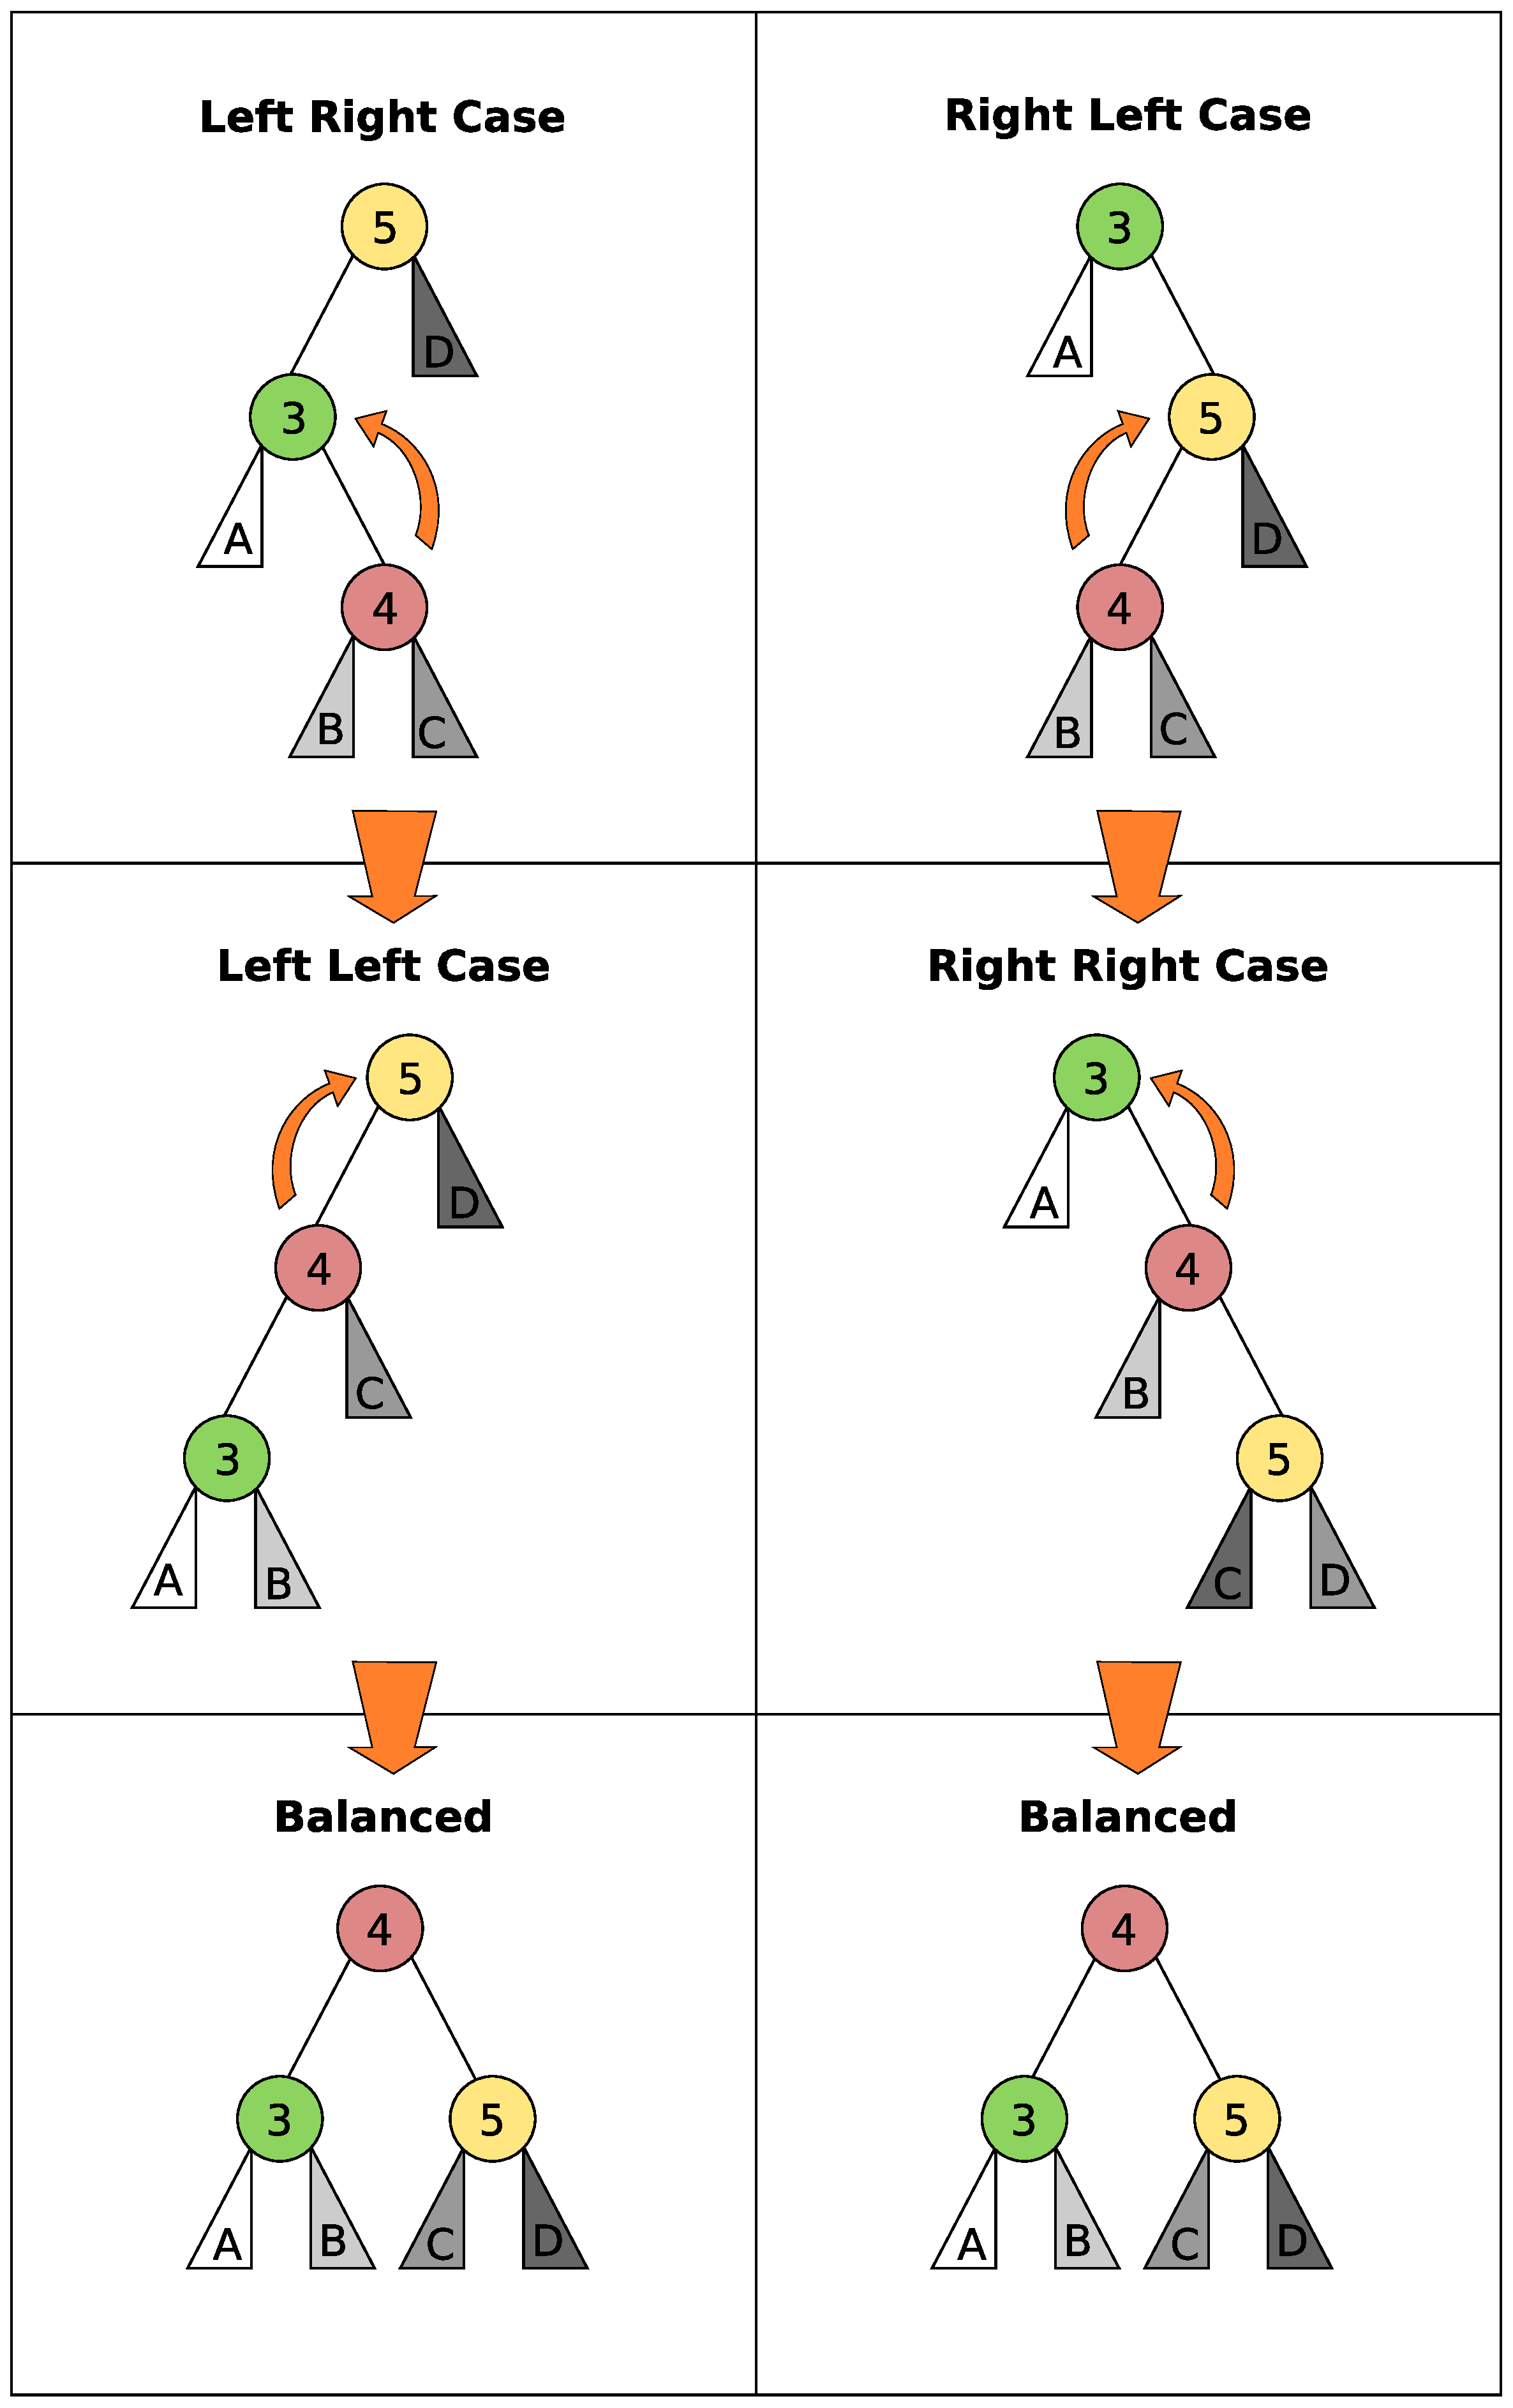
\includegraphics[height=16cm]{chapter13/AVL_Tree_Rebalancing.eps}
		%\begin{figure}
		%\centering
		%\def\svgwidth{\columnwidth}
		%\includegraphic{AVL_Tree_Rebalancing.eps}
		%\end{figure}

	\item	the procedure $\proc{AVL-Insert}(x, z)$ consist of $\proc{BST-Tree-Insert}(T, z)$ and $\proc{Balance}(x)$
	\item	$\proc{BST-Tree-Insert}(T, z)$: $\mathcal{O}(\log{n})$ \\
		$\proc{Balance}(x)$: $\mathcal{O}(\log{n})$ \\
		$\proc{AVL-Insert}(x, z)$ Total: $\mathcal{O}(\log{n})$
\end{enumerate}


\subsection*{Problem 13-4 Treaps}
\begin{enumerate}
	\item	对于一棵BST,可以对每个节点进行Rotation,所有这些BST与原始的BST都是同构的,然而在Treap中,这棵树要满足Heap的性质,所以不能进行Rotation,即这棵BST是确定唯一的
	\item	对于所有节点的priority序列,每一种排列都唯一的对应一种Treap,即所有节点以一种排列顺序插入所形成的BST,因为所有的节点的priority都是随机产生的,所以Treap的本质就是Randomly built binary search trees,所以the expected height of a treap is $\Theta(\log{n})$
	\item	the procedure $\proc{Treap-Insert}$ consist of $\proc{BST-Tree-Insert}$ and $\proc{Heap-Increase-Key}$ by $\proc{Rotation}$
	\item	$\proc{BST-Tree-Insert}$: $\mathcal{O}(\log{n})$ \\
		$\proc{Heap-Increase-Key}$: $\mathcal{O}(\log{n})$ ($\proc{Rotation}$: $\mathcal{O}(1)$) \\
		$\proc{Treap-Insert}$ Total: $\mathcal{O}(\log{n})$
	\item	对于一个leaf node $x$,可以归纳,每次对于$x$进行一次Rotation,其$C + D$会增加1,归纳过程如图 \\
		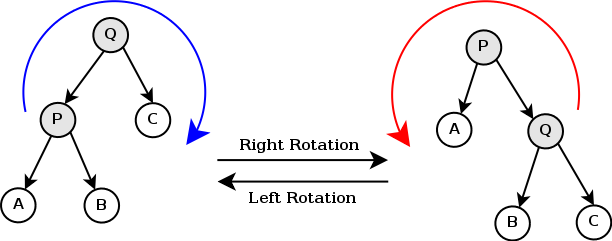
\includegraphics[width=10cm]{chapter13/Tree_rotation.png} \\
		对于Right-Rotation,设节点$x$为$P$,$A, B$分别为$x$的左右两棵子树,$Q$是$P$的parent,$C$是$Q$的右子树,原始的$C + D = left\_spine(B) + right\_spine(A)$,经过Right-Rotation后,$C' + D' = right\_spine(A) + 1 + left\_spine(B)$ \\
		同理,Left-Rotation亦是如此,即对于插入树中的节点$x$,其Rotation的次数等于$C + D$
	\item	(Omit!)
	\item	\begin{equation} \notag
			Pr\{X_{ik} = 1\} = \frac{(k - i - 1)!}{(k - i + 1)!} = \frac{1}{(k - i + 1)(k - i)}
		\end{equation}
	\item	\begin{equation} \notag
			E[C] = \sum_{i = 1}^{k - 1} Pr\{X_{ik} = 1\} = \sum_{i = 1}^{k - 1} \frac{1}{(k - i + 1)(k - i)} = \sum_{j = 1}^{k - 1} \frac{1}{j(j + 1)} = 1 - \frac{1}{k}
		\end{equation}
	\item	由对称性,令$k = n - k + 1$即可,即
		\begin{equation} \notag
			E[D] = 1 - \frac{1}{n - k + 1}
		\end{equation}
	\item	因为$E[C + D] = E[C] + E[D] < 2$,所以当向Treap中插入一个节点时,期望的Rotation次数小于2
\end{enumerate}



\pagebreak



\section*{IV Advanced Design and Analysis Techniques}
\pagebreak

\section*{Chapter 14}

\pagebreak

\section*{Chapter 15}

\subsection*{15-1 Longest simple path in a directed acyclic graph}
\noindent Let $f(i)$ be the longest distant from vertex $s$ to vertex $i$ \\
Recursive formulation:
\begin{equation} \notag
	f(i) = \max_{(j, i) \in E}\{f(j) + d_{ji}\} \\
\end{equation}
initial case:
\begin{equation} \notag
	f(s) = 0
\end{equation}
Visit every vertex in Graph $G$ by topological order \\
Running time: $\mathcal{O}(V + E)$


\subsection*{15-2 Longest palindrome subsequence}
\noindent Let $f(i, j)$ be the length of the longest palindrome subsequence from the $i$th character to the $j$th character \\
Recursive formulation:
\begin{equation} \notag
	f(i, j) = \begin{cases}
		1,	& \mbox{if } i = j \\
		0,	& \mbox{if } i > j \\
		f(i + 1, j - 1) + 2,	& \mbox{if } a_i = a_j \\
		\max\{f(i + 1, j), f(i, j - 1)\},	& \mbox{otherwise} \\
	\end{cases}
\end{equation}
Running time: $\mathcal{O}(n^2)$


\subsection*{15-3 Bitonic euclidean traveling-salesman problem}
\noindent First, sort the points by $x$-coordinate, <$P_1, P_2, .., P_n$> $(x_{P_i} < x_{P_{i + 1}})$ \\
Let $P_{i, j}$ $(i < j)$ denote the bitonic path: $P_i \xrightarrow{left} P_1 \xrightarrow{right} P_j$ (a vertex-disjoint path) \\
It means that the bitonic path $P_{i, j}$ $(i < j)$ includes all vertices $P_1, P_2, \cdots, P_j$ \\
Let $f(i, j)$ $(i \leq j \leq n)$ be the length of the shortest bitonic path $P_(i, j)$ \\
Recursive formulation:
\begin{equation} \notag
\begin{cases}
	f(i, j) = f(i, j - 1) + \abs{P_{j - 1, j}} & \mbox{if } (i < j - 1) \\
	f(i - 1, i) = \displaystyle{\min_{1 \leq k < i - 1}} \{f(k, i - 1) + \abs{P_k P_i}\} \\
	f(i, i) = f(i - 1, i) + \abs{P_{i - 1}P_i}
\end{cases}
\end{equation}
initial case:
\begin{equation} \notag
	f(1, 2) = \abs{P_1 P_2}
\end{equation}
Running time: $\mathcal{O}(n^2)$


\subsection*{15-4 Printing neatly}
\noindent Let $cost(i, j)$ denote the number of extra space characters at the end of the line which includes the $i \cdots j$-th word \\
Therefore,
\begin{equation} \notag
	cost(i, j) = \begin{cases}
		0,	& \mbox{if } j = n \mbox{ and } M - j + i - \displaystyle{\sum^{j}_{k = i}} l_k \geq 0 \\
		\infty,	& \mbox{if } M - j + i - \displaystyle{\sum^{j}_{k = i}} l_k < 0 \\
		\displaystyle{(M - j + i - \sum^{j}_{k = i} l_k)^3},	& \mbox{otherwise}
	\end{cases}
\end{equation}
Let $f(i)$ be the minimum number of extra space characters after placing first $i$th words \\
Recursive formulation:
\begin{equation} \notag
	f(i) = \min_{0 \leq j < i}\{f(j) + cost(j + 1, i)\}
\end{equation}
initial case:
\begin{equation} \notag
	f(0) = 0
\end{equation}
Running time: $\mathcal{O}(n^2)$ \\
Space: $\mathcal{O}(n)$


\subsection*{15-5 Edit distance}
\begin{enumerate}
	\item	Let $X_i = x[1 .. i]$ and $Y_i = y[1 .. y]$ and $f(i ,j)$ denote the minimum cost of transformating $X_i$ to $Y_j$ \\
		Recursive formulation:
		\begin{equation} \notag
			f(i, j) = \min \begin{cases}
				f(i - 1, j - 1) + cost(copy),	& \mbox{if } x[i] = y[j] \\
				f(i - 1, j - 1) + cost(replace),& \mbox{if } x[i] \neq y[j] \\
				f(i - 1, j) + cost(delete) \\
				f(i, j - 1) + cost(insert) \\
				f(i - 2, j - 2) + cost(twiddle),& \mbox{if } i, j \geq 2,x[i] = y[j - 1],\mbox{and } x[i - 1] = y[j] \\
				\displaystyle{\min_{0 \leq k < m}} \{f(k, n)\} + cost(kill), & \mbox{if } i = m \mbox{ and } j = n
			\end{cases}
		\end{equation}
		initial case:
		\begin{equation} \notag
			f(0, 0) = 0
		\end{equation}
		Running time and Space: $\mathcal{O}(nm)$
	\item	\begin{equation} \notag
		\begin{aligned}
			&cost(copy) = -1 \\
			&cost(replace) = 1 \\
			&cost(delete) = 2 \\
			&cost(insert) = 2
		\end{aligned}
		\end{equation}
		maximize $\rightarrow$ minimize
\end{enumerate}


\subsection*{15-6 Planning a company party}
\noindent Let $f(x, 0)$ denote the maximum sum of the conviviality ratings of the guests when the emplyee $x$ doesn't attend the party and $f(x, 1)$ denote the maximum sum of the conviviality ratings of the guests when the emplyee $x$ attends the party \\
Recursive formulation:
\begin{equation} \notag
\begin{aligned}
	&f(x, 0) = \sum_{y \in Son\{x\}} \max\{f(y, 0), f(y, 1)\} \\
	&f(x, 1) = \sum_{y \in Son\{x\}} f(y, 0) + rating(x)
\end{aligned}
\end{equation}
initial case: if $x$ is a leaf,
\begin{equation} \notag
\begin{aligned}
	&f(x, 0) = 0 \\
	&f(x, 1) = rating(x)
\end{aligned}
\end{equation}
Running time: $\mathcal{O}(V + E)$


\subsection*{15-7 Viterbi algorithm}
\begin{enumerate}
	\item	Let $f(x, i)$ denote whether there exist a path in $G$ that begins at $x$ and has a sequence <$\sigma_1, \sigma_2, \cdots, \sigma_i$> as it label \\
		Recursive formulation:
		\begin{equation} \notag
			f(x, i) = \bigvee_{y \mbox{ s.t. } \sigma(y, x) = \sigma_i } f(y, i - 1)
		\end{equation}
		initial case:
		\begin{equation} \notag
			f(x, 0) = true
		\end{equation}
		Running time: $\mathcal{O}(kn^2)$
	\item	Let $f(x, i)$ denote the maximum probability of a path in $G$ that begins at $x$ and has a sequence <$\sigma_1, \sigma_2, \cdots, \sigma_i$> as it label \\
		Recursive formulation:
		\begin{equation} \notag
			f(x, i) = \max_{y \mbox{ s.t. } \sigma(y, x) = \sigma_i}\{f(y, i - 1) \cdot p(y, x)\}
		\end{equation}
		Running time: $\mathcal{O}(kn^2)$
\end{enumerate}


\subsection*{15-8 Image compression by seam carving}
\begin{enumerate}
	\item	$\mathcal{O}(3^m)$
	\item	Let $f(i, j)$ denote the seam with the lowest disruption measure of $i \times j$ array $A[1..i, 1..j]$ \\
		Recursive formulation:
		\begin{equation} \notag
			f(i, j) = \min\{f(i - 1, j - 1), f(i - 1, j), f(i - 1, j + 1)\} + d[i, j]
		\end{equation}
		The answer is find the $i$ such that minimize $f(m, i)$ \\
		Running time: $\mathcal{O}(nm)$
\end{enumerate}


\subsection*{Problem 15-9 Breaking a string}
\noindent Let $L[0] = 0$ and $L[m + 1] =  n$ \\
Let $f(i, j)$ denote the lowest cost of breaks that breaking every break points in $L[i..j - 1]$ \\
Recursive formulation:
\begin{equation} \notag
	f(i, j) = \min_{i < k < j} \{f(i, k) + f(k, j)\} + (L[j] - L[i])
\end{equation} 
initial case:
\begin{equation} \notag
	f(i, i + 1) = 0
\end{equation}
The answer is $f(0, m + 1)$
Running time: $\mathcal{O}(m^3)$


\subsection*{Problem 15-10 Planning an investment strategy}
\begin{enumerate}
	\item	(Explicit)
	\item	Let $f(k, i)$ denote in $k$ years and we inveset the $i$th investment at the $k$th year, the maximum amount of the monney \\
		Recursive formualation:
		\begin{equation} \notag
			f(k, i) = \max_{j \neq i} \{f(k - 1, i) - f_1, f(k - 1, j) - f_2\} + d \cdot r_{ik}
		\end{equation}
	\item	Running time: $\mathcal{O}(years \cdot inverstments^2) = \mathcal{O}(n^2)$
	\item	(Omit!)
\end{enumerate}


\subsection*{Problem 15-11 Inventory planning}
\noindent Let $D(x) = \displaystyle{\sum_{i = 1}^{x}} d_i$ and $D(0) = 0$, therefore, $D(n) = D$ \\
Let $f(i, j)$ denote the minimum cost of first $i$th month that manufactured $j$ machines \\
Recursive formulation:
\begin{equation} \notag
	f(i, j) = \min_{j \geq k \geq D(i - 1)}\{f(i - 1, k) + \max\{0, j - k - m\} \cdot c\} + h(j - D(i)), \mbox{ for } D \geq j \geq D(i)
\end{equation}
The answer is $f(n, D)$ \\
Running time: $\mathcal{O}(nD^2)$


\subsection*{Problem 15-12 Signing free-agent baseball players}
\noindent For every free-agent player $x$, let $pos(x)$ denote the player's position, $cost(x)$ denote the amount of money it will cost to sign the player, and $vorp(x)$ denote the player's VORP \\
Let $f(i, j)$ denote the maximum total VORP of the players signed for first $i$ position and used $j$ money \\
Recursive formulation:
\begin{equation} \notag
	f(i, j) = \max_{k \mbox{ s.t. } pos(k) = i} \{f(i - 1, j), f(i - 1, j - cost(k)) + vorp(k)\}
\end{equation}
The answer is $f(N, X)$ \\
Running time: $\mathcal{O}(\max(N, P)\cdot X)$



\pagebreak


\end{document}

